\chapter{非均匀介质中带有 Lipschitz 界面的时谐 Maxwell 方程虚单元方法}
本章节我们介绍在非均匀介质中带有
Lipschitz 界面的时谐 Maxwell
方程的虚单元方法,在本方法中,我们对网格要求较低,允许非常窄的单元,
这使得我们可以通过简单的方式生成界面拟合网格。
我们假设网格中每个单元存在一个虚网格,基于这种虚网格技术,我们证明了
提出的方法在理论上可保证对于仅具有 $\bfH^{\theta}$
正则性($\theta\in(1/2,1]$)的解仍能获得鲁棒的最优收敛性。
且多边形单元形状可以高度各向异性,
我们建立了一个显式公式来描述形状正则性与解正则性之间的关系。
此外,我们证明了对于不定时谐 Maxwell 问题而言,
稳定化项的引入是获得数值解最优收敛性所必需的。

\section{时谐 Maxwell 方程}
%设 $\bv = [v_1,v_2]^T$ 为一个二维矢量场,$v$ 为一个标量函数,
%定义旋度算子 $\rot \bv = \partial_{x_1} v_2 - \partial_{x_2} v_1$,以及广义旋度算子 $\brot v = [\partial_{x_2}v , -\partial_{x_1}v]^T$。
令 $\Omega \subseteq \mathbb{R}^2$ 为一个有界区域。
二维时谐 Maxwell 方程形式如下:
\begin{equation}
\label{model0}
\brot \mu^{-1} \rot \bu - \omega^2(\epsilon + i \sigma/\omega) \bu = \bsf, ~~~~ \text{ in } ~ \Omega,
\end{equation}
其中 $i = \sqrt{-1}$,$\bsf \in \bH(\ddiv^0;\Omega)$ 表示源项。
本文考虑完美电导体边界条件(PEBC),即 $\bu\cdot\bt = 0$。
方程中的参数 $\mu > 0$、$\omega > 0$、$\epsilon \geq 0$、$\sigma \geq 0$
分别表示磁导率、角频率、介电常数和电导率。

若 $\sigma \neq 0$,则 \eqref{model2} 在 $\bH(\rot;\Omega)$ 空间中是强制的,
这一点可参考文献 \cite{1992Monk,2003GopalakrishnanPasciak},以及文献 \cite{2019BonazzoliDoleanGrahamSpenceTournier} 的引理 2.5 的证明。
在这种情况下,可通过 Lax-Milgram 引理的标准方法进行分析。
当 $\sigma$ 和 $\epsilon$ 均为零时,为了保证问题的适定性,需要显式地施加 $\ddiv \bu = 0$ 这一约束条件。
而当 $\omega^2(\epsilon + i \sigma/\omega)\neq 0$ 时,由于 $\ddiv\bsf = 0$ 以及 $\ddiv\brot = 0$,这一约束实际上是隐式施加的。

在本章,我们考虑 $\sigma = 0$ 且 $\omega^2 \epsilon > 0$ 的情况,此时
当方程 \eqref{model0} 施加阻抗边界条件,且 $\omega^2\epsilon$ 不是
$\brot\mu^{-1}\rot$ 算子的特征值时,
方程
解存在唯一,这一结论可参考文献 \cite{2003Monk} 的定理 4.17。
然而,在 PEBC 边界条件下,需要额外的假设,我们在假设 \ref{assum_eigen} 中进行了讨论。

在非均匀介质问题中,
计算区域 $\Omega$ 可能是多个子区域的并集,
见图 \ref{fig:example12}、\ref{fig:interfacedoublecircle} 和
\ref{fig:fivelayerspolymesh},
每个子区域的电磁特性可能不同,
这在方程中体现为参数
$\mu$、$\epsilon$ 和 $\sigma$ 是不连续的常数。
为便于讨论,本文仅考虑 $\Omega$ 被一条可能非光滑的闭合界面 $\Gamma$ 分割为 $\Omega^+$ 和 $\Omega^-$ 的情形。

令 $\alpha=\mu^{-1}$,$\beta = \omega^2\epsilon$,它们在 $\Omega^+$ 和 $\Omega^-$ 上分别取常数:
\begin{equation*}
\alpha|_{\Omega^{\pm}}=\alpha^{\pm}, \quad \beta|_{\Omega^{\pm}}=\beta^{\pm}.
\end{equation*}
此时,方程 \eqref{model0} 可重写为:
\begin{equation}
\label{model1}
\brot \alpha \rot \bu - \beta \bu = \bsf, ~~~~ \text{在} ~ \Omega.
\end{equation}
相应的变分形式为:
\begin{equation}
\label{model2}
a(\bu,\bv) := (\alpha\rot \bu, \rot \bv)_{\Omega} - (\beta \bu, \bv)_{\Omega} = (\bsf, \bv), ~~~~ \forall \bv\in \bH_0(\rot;\Omega).
\end{equation}
界面条件如下
\begin{equation}
\label{interfaceCond}
[\bu\cdot\bt]_{\Gamma} := (\bu^+\cdot\bt-\bu^-\cdot\bt)|_{\Gamma} = 0, ~~~~
[\alpha \rot \bu]_{\Gamma} := (\alpha \rot \bu^+ - \alpha \rot \bu^-)|_{\Gamma} = 0.
\end{equation}
%由于 $\bsf \in \bH(\ddiv;\Omega)$,可进一步推出 $[\beta \bu \cdot\bfn]_{\Gamma} = 0$,但本文不显式使用该条件。

%关于 $\Gamma$ 的几何特性,请参考假设 \ref{assum_geo},
%其中允许 $\Gamma$ 存在拐点,但拐角不能任意小。




%%%%%%%%%%%%%%%%%%%%%%%%%%%%%%%%%%%%%%%%%%%%%%%%%%%%%%%%

\section{基本假设}
本文考虑满足以下条件的Lipschitz界面 $\Gamma$:
\begin{assumption}
\label{assum_geo}
界面满足以下条件:
\begin{itemize}
\item[(I1)]\label{asp:I1} 界面不与自身相交;
\item[(I2)]\label{asp:I2} 正则性质:存在常数$c_0$使得
\begin{equation}
\label{Dregular}
|B(\bfx,r)\cap \Omega^{\pm}| \ge c_0 r^2 ~~~ \forall \bfx \in \Omega^{\pm}, ~~ r\in[0,1],
\end{equation}
其中$B(\bfx,r)$表示以$\bfx$为中心、$r$为半径的球。
\end{itemize}
\end{assumption}
%注意到假设\ref{assum_geo}中的\hyperref[asp:I1]{(I1)}本质上意味着$\Gamma$与$\partial\Omega$的夹角需下界远离$0$且上界远离$\pi$。

设$\mathcal{T}_h$为拟合界面和区域边界的多边形网格,即每个单元仅位于界面的一侧。
由于本文对多边形单元形状要求较低,
$\mathcal{T}_h$可以使用简单的方式生成,如图\ref{fig:NonConfMesh}所示。

\begin{figure}[h]
\centering
\begin{subfigure}{.2\textwidth}
    \includegraphics[width=1in]{./figures/maxwell/UnfitMesh1}
    % \caption{Type I:5 tetrahedra}
     \label{fig:UnfitMesh1} %% label for first subfigure
\end{subfigure}
%%
 \begin{subfigure}{.2\textwidth}
     \includegraphics[width=1.1in]{./figures/maxwell/UnfitMesh2}
     %\caption{Type II: 24 tetrahedra}
     \label{fig:UnfitMesh2} %% label for first subfigure
\end{subfigure}
%%%%%
\begin{subfigure}{.2\textwidth}
    \includegraphics[width=1in]{./figures/maxwell/NonConfMesh1}
    % \caption{Type I:5 tetrahedra}
     \label{fig:NonConfMesh1} %% label for first subfigure
\end{subfigure}
%%
 \begin{subfigure}{.2\textwidth}
     \includegraphics[width=1in]{./figures/maxwell/NonConfMesh2}
     %\caption{Type II: 24 tetrahedra}
     \label{fig:NonConfMesh2} %% label for first subfigure
\end{subfigure}
     \caption{左侧两张图(半结构化网格):笛卡尔网格被圆形界面切割,
         一些单元被分割成两个多边形以逼近界面,
     右侧两张图(非匹配网格):正方形界面将区域划分为两个子区域,
     它们分别被不同的网格离散化,
     但这两个网格在界面处可能不匹配,
 由此会在界面附近产生形状极为复杂的多边形单元.}
  \label{fig:NonConfMesh} %% label for entire figure
\end{figure}

设$\Gamma_h$为通过连接$\Gamma$与单元边的交点及 $\Gamma$ 的角点形成的折线,
是界面 $\Gamma$ 的近似。
此折线将$\Omega$划分为近似子区域$\Omega^{\pm}_h$。
令$\alpha_h$和$\beta_h$ 为 $\Omega_h^{\pm}$ 上的分片常数,分别对应于
$\alpha$和$\beta$,即:$\alpha_h|_{\Omega^{\pm}_h} =
\alpha|_{\Omega^{\pm}}$和$\beta_h|_{\Omega^{\pm}_h} = \beta|_{\Omega^{\pm}}$。
注意$\Gamma_h$由网格单元边构成(见图\ref{fig:interfelem})。
$\Gamma_h$与$\Gamma$之间存在不匹配的区域,定义为$(\Omega^+_h\cap \Omega^-)\cup
(\Omega^-_h\cap \Omega^+)$,需在分析中谨慎处理。
为此,参照\cite{2010LiMelenkWohlmuthZou}引入界面邻近区域:
\begin{equation}
\label{OmegaGamma}
\Omega^{\Gamma}_{\epsilon} = \{ \bfx\in \Omega: \mathrm{dist}(\bfx,\Gamma)< \epsilon \},
\end{equation}
{在此区域上,离散变分形式的系数$\alpha_h$和$\beta_h$可能与连续形式的$\alpha$和$\beta$不同。}
关于不匹配区域,我们作如下假设(该假设的几何解释见图\ref{fig:interfelem}右图):
\begin{assumption}
\label{interf_eps}
存在与网格无关、仅依赖于$\Gamma$的常数$\epsilon>0$,使得
\begin{equation}
\label{interf_eps_eq}
(\Omega^+_h\cap \Omega^-)\cup (\Omega^-_h\cap \Omega^+) \subseteq \Omega^{\Gamma}_{\epsilon h^2}.
\end{equation}
\end{assumption}

\begin{figure}[h]
\centering
\begin{subfigure}{.2\textwidth}
\includegraphics[width=1.05in]{./figures/maxwell/interfelem1}
\label{fig:interfelem1}
\end{subfigure}
%%
\begin{subfigure}{.2\textwidth}
\includegraphics[width=1.05in]{./figures/maxwell/interfelem3}
\label{fig:interfelem2}
\end{subfigure}
%%
\begin{subfigure}{.2\textwidth}
\includegraphics[width=1.05in]{./figures/maxwell/interfelem2}
\label{fig:interfelem3}
\end{subfigure}
%%
\caption{左:界面(红色)将单元$K$切割为两个子单元;通过连接交点构造近似线段$\Gamma^K_h$(蓝色)。
中:分段光滑界面曲线的多边形近似$\Gamma^K_h$。
右:$\Omega^{\pm}$与$\Omega^{\pm}_h$的不匹配区域,该区域包含在薄带$\Omega_{\epsilon
h^2}$中.}
\label{fig:interfelem}
\end{figure}

下面引入 $\Omega^{\pm}$ 上的分片 Sobolev 空间。
%设 $H^s(D)$、$\bH^s(D):= H^s(D, \mathbb{R}^2)$($s\ge 0$)为标准(向量)Sobolev空间。
%{
%$\bH^s(\rot;D)$表示满足$\rot \bu \in H^s(D)$的$\bu\in \bH^s(D)$空间:
%$$
%\bH^s(\rot;D) = \{ \bu \in \bH^s(D): \rot \bu \in H^s(D) \}.
%$$
%}
对于与$\Gamma$相交的区域$D\subseteq\Omega$,定义分片Sobolev空间$H^s(D^{\pm})$,其范数为
$$
\| v \|_{s,D^{\pm}} = \| v \|_{s,D^{+}} + \| v \|_{s,D^{-}} ~~~ \forall v\in H^s(D^{\pm}).
$$
类似地定义$\bH^s(\Omega^{\pm})$。进一步引入:
\begin{equation*}
\begin{split}
& \bH^s(\rot;D^{\pm}) = \{ \bv\in [L^2(D)]^2~:~ \bv|_{D^{r}} \in \bH^s(\rot;D^{r}), ~ r = +~\text{或} - \},\\
& \|\bv\|_{s,\rot;D^{\pm}} = \|\bv\|_{s,\rot;D^{+}} + \|\bv\|_{s,\rot;D^{-}},
\end{split}
\end{equation*}

为研究问题 \eqref{model1} 的适定性,
考虑如下椭圆方程:
\begin{equation}
\begin{split}
\label{H1eqn}
& \ddiv(a\nabla u) = f ~~ \text{in} ~~ \Omega, ~~~~ [u]_{\Gamma} =0, ~ [a\nabla
u\cdot\bfn]_{\Gamma}=0 ~ \text{on} ~ \Gamma,\\
& u=0 ~~ \text{or} ~~ a\nabla u \cdot \bfn =0 ~ \text{on} ~~ \partial\Omega,
\end{split}
\end{equation}
根据文献\cite{2016Ciarlet}定理16,在条件\hyperref[asp:I1]{(I1)}下,解$u\in H^{1+\theta}_0(\Omega^{\pm})$,$\theta\in(1/2,1]$。
基于这样的正则性结果,我们建立如下嵌入关系:
\begin{lemma}
\label{lem_embd_1}
在假设 \ref{assum_geo} 中的 \hyperref[asp:I1]{(I1)} 条件下,存在 $\theta\in(1/2,1]$,使得
\begin{equation}
\label{lem_embd_1_eq0}
\bH_0(\rot;\Omega)\cap \bH(\beta, \ddiv;\Omega) \hookrightarrow \bH^{\theta}(\Omega^{\pm}).
\end{equation}
此外,
如果 $\Omega$ 关于某一点 $\bfb_{\Omega}$ 是星形的,则
对于任意 $\bu\in \bH_0(\rot;\Omega)\cap \bH(\beta, \ddiv;\Omega)$,
以下估计成立:
\begin{equation}
  \label{lem_embd_1_eq01}
  \| \bu \|_{0,\Omega} 
  \le 2 \sqrt{\varpi}  h^2_{\Omega}|\Omega|^{-1/2} \|\rot \bu \|_{0,\Omega} 
  + \beta_{\min}^{-1} ( \sqrt{\pi} j_0)^{-1} |\Omega|^{1/2} \|\ddiv(\beta \bu) \|_{0,\Omega},
  \end{equation}
其中 $h_{\Omega}$ 是 $\Omega$ 的直径,$|\Omega|$ 是面积,
$\beta_{\max}=\max\{\beta^+,\beta^-\}$,$\beta_{\min}=\min\{\beta^+,\beta^-\}$,
且 $\varpi = \beta_{\max}/\beta_{\min}$。
%如果 $\Omega$ 是凸多边形或具有光滑边界,则 $\theta=1$。
\end{lemma}
\begin{proof}
由于 $\bu\in \bH_0(\rot;\Omega)$,我们首先构造一个函数 $\phi$ 满足
\begin{equation}
\label{lem_embd_1_eq1_1}
\rot( \beta^{-1} \, \brot \phi ) = - \ddiv\left( \beta^{-1} \nabla \phi \right) =  \rot \bu , ~~~~ [\phi]_{\Gamma} = \mathbf{0}, ~~~~ [ \beta^{-1} \nabla  \phi \cdot \bfn ]_{\Gamma} = 0, 
\end{equation}
且满足在 $\partial\Omega$ 上,
$
\beta^{-1} \brot \phi  \cdot \bt = \beta^{-1} \nabla \phi \cdot \bfn = 0
$。
为了保证唯一性,我们施加积分为零的条件: $\int_{\Omega}\phi \dd \bfx = 0$。
同样,由于 $\bu\in \bH(\beta, \ddiv;\Omega)$,我们引入另一个函数 $\psi$ 满足
\begin{equation}
\label{lem_embd_1_eq1_2}
-\ddiv(\beta \nabla \psi ) =  -\ddiv( \beta \bu ), ~~~~ [\psi]_{\Gamma} = \mathbf{0}, ~~~~ [ \beta \nabla \psi \cdot \bfn ]_{\Gamma} = 0,
\end{equation}
满足在 $\partial\Omega$ 上,
$
%\nabla\bfpsi\cdot\bfn = \mathbf{ 0}
\psi = 0
$ 。
下面证明如下等式成立:
\begin{equation}
\label{lem_embd_1_eq2}
\bu = \beta^{-1} \brot \phi + \nabla \psi.
\end{equation}
记 $\bfTheta = \bu - \beta^{-1} \brot \phi - \nabla \psi$,根据方程
\eqref{lem_embd_1_eq1_1} 和 \eqref{lem_embd_1_eq1_2} 可得 $\rot( \bfTheta )=
\ddiv(\beta \bfTheta ) = \mathbf{ 0}$。
此外,根据边界条件可知 $\bfTheta\cdot\bt = \bu\cdot\bt - \beta^{-1} \nabla \phi \cdot \bfn  - \nabla \psi \cdot \bt = 0$,
这意味着 $\bfTheta \in \bH_0(\rot^0;\Omega)$。
根据 de Rham 复形,存在 $\varphi\in H^1_0(\Omega)$ 使得 $\bfTheta = \nabla
\varphi$,满足
\begin{equation}
\label{lem_embd_1_eq2_1}
\ddiv( \beta \nabla\varphi ) = \mathbf{ 0} ~~~ \text{在} ~  \Omega 中,
\end{equation}
所以 $\bfTheta =  \nabla\varphi =  \mathbf{ 0}$,\eqref{lem_embd_1_eq2} 成立。
此外,根据 \eqref{H1eqn} 中描述的界面问题的椭圆正则性可知
$\phi\in H^{1+\theta}(\Omega^{\pm})$,$\psi\in H^{1+\theta}(\Omega^{\pm})$,且
$$
\| \phi \|_{1+\theta,\Omega^{\pm}}  \lesssim  \|  \rot \bu  \|_{0,\Omega} ~~~ \text{且} ~~~ \| \psi \|_{1+\theta,\Omega^{\pm}}  \lesssim \| \ddiv( \beta \bu )  \|_{0,\Omega}.
$$ 
因此,根据 \eqref{lem_embd_1_eq2},我们有 $\bu \in \bH^{\theta}(\Omega^{\pm})$,且满足 \eqref{lem_embd_1_eq0} 中的有界性。

现在,我们证明 \eqref{lem_embd_1_eq01}。
将 \eqref{lem_embd_1_eq1_1} 乘以 $\phi$,利用分部积分
以及\eqref{eq:Poincare-Friedrichs1} 我们得到
$$
  \|\beta^{-1/2}\nabla\phi\|^2_{L^2(\Omega)} = (\rot\bu, \phi)_{\Omega}
  \le \| \rot\bu \|_{0,\Omega} \|\phi\|_{0,\Omega}
  \le 2 h^2_{\Omega}|\Omega|^{-1/2}  \|\nabla \phi\|_{0,\Omega} \| \rot\bu \|_{0,\Omega}.
$$
然后,注意到 $\|\nabla \phi\|_{0,\Omega} \le \beta_{\max}^{1/2} \| \beta^{-1/2} \nabla \phi\|_{0,\Omega}$,
我们在上述两边各消去一个 $\| \beta^{-1} \nabla \phi\|_{0,\Omega}$ 项,得到
\begin{equation}
  \label{lem_embd_1_eq3}
  \|\beta^{-1}\nabla\phi\|_{L^2(\Omega)} \le \beta_{\min}^{-1/2} \|\beta^{-1/2}\nabla\phi\|_{L^2(\Omega)} 
  \le 2 \sqrt{\varpi}  h^2_{\Omega}|\Omega|^{-1/2} \| \rot\bu \|_{0,\Omega}.
\end{equation}
对于 $\psi$,使用迹零的 Poincar\'e 不等式 \eqref{eq:Poincare-Friedrichs2}
我们得到
$$
\|  \psi \|_{0,\Omega} \le ( \sqrt{\pi} j_0)^{-1} |\Omega|^{1/2} \| \nabla \psi \|_{0,\Omega},
$$
然后,将 \eqref{lem_embd_1_eq1_2} 乘以 $\psi$ 并利用分部积分,我们得到
\begin{equation}
  \label{lem_embd_1_eq4}
\| \beta^{1/2} \nabla \psi \|^2_{0,\Omega} 
\le \| \ddiv(\beta\bu) \|_{0,\Omega} \| \psi \|_{0,\Omega}
\le ( \sqrt{\pi} j_0)^{-1} |\Omega|^{1/2} \| \nabla \psi \|_{0,\Omega} \| \ddiv(\beta\bu) \|_{0,\Omega},
\end{equation}
然后,我们在上述两边各消去一个 $\| \nabla \psi \|^2_{0,\Omega}$ 项,
再根据 \eqref{lem_embd_1_eq2} 和 \eqref{lem_embd_1_eq3},得到所需的估计 \eqref{lem_embd_1_eq01}。
\end{proof}
\vspace{20pt}

注意若 $\beta$ 恰好是 $\brot \alpha \rot$ 算子的特征值,那么在 PEBC 下,模型问题
\eqref{model1}
可能没有唯一解。所以为了保证解的唯一性,作如下假设:
\begin{assumption}
\label{assum_eigen}
$\beta$不是$\bf{rot}\alpha\rot$算子的特征值,即不存在$\bu \in \bH_0(\rot;\Omega)$使得$\bf{rot}\alpha\rot \bu = \beta \bu$。
\end{assumption}
\begin{remark}
特征值会依赖于 $\Omega$ 的形状以及界面 $\Gamma$,
假设 $\Omega$ 的直径为 $h_{\Omega}$,并且关于半径为 $r_{\Omega}\ge \nu h_{\Omega}$ 的球是星形的,其中 $\nu\in(0,1)$。  
%记 $\beta_{\max}=\max\{\beta^+,\beta^-\}$,$\beta_{\min}=\min\{\beta^+,\beta^-\}$,且 $\varpi = \beta_{\max}/\beta_{\min}$。  
根据引理 \ref{lem_embd_1} 以及 $\bu \in \bfK(\beta;\Omega)$,我们得到 Poincar\'e 不等式:
$$
\| \bu \|_{0,\Omega} \le 2 \sqrt{\varpi} h^2_{\Omega}|\Omega|^{-1/2} \| \rot\bu \|_{0,\Omega} 
\le \sqrt{\varpi/\pi} \nu^{-1} h_{\Omega} \| \rot\bu \|_{0,\Omega}.
$$
可以看到,如果 $\Omega$ 越来越窄,即: $\nu\rightarrow 0$ 但 $h_{\Omega}$ 不为 0 ,
上述不等式右端的常数可能会趋于无穷大。  
因此,如果我们固定 $\nu$ 并使 $\Omega$ 足够小,使得
\begin{equation}
  \label{dom_small_eq1}
  h_{\Omega} <  \nu \sqrt{ \frac{\alpha_{\min}}{\beta_{\max}} \frac{\pi}{\varpi} },
\end{equation}
则有
\begin{equation}
  \label{dom_small_eq2}
\| \sqrt{\alpha} \rot \bu \|^2_{0,\Omega} \ge \alpha_{\min} \| \rot \bu \|^2_{0,\Omega} > \beta_{\max} \| \bu \|^2_{0,\Omega},
\end{equation}
这保证了假设 \ref{assum_eigen} 的成立。
\end{remark}

定义$\beta$-divergence free 的子空间:
\begin{equation}
\label{div_free}
\bfK(\beta;\Omega) = \bH_0(\rot;\Omega) \cap \bH(\beta,\ddiv^0;\Omega) .
\end{equation}
由引理\ref{lem_embd_1}可得嵌入关系:
\begin{equation}
\label{lem_embd_2}
\bfK(\beta;\Omega)  \hookrightarrow \bH^{\theta}(\Omega^{\pm}),
\end{equation}
其中$\theta$由引理\ref{lem_embd_1}给出。




\section{网格假设}
\label{sec:mesh_assump}

在本节中,我们将介绍关于多边形单元形状的假设,
这些假设与文献中的经典假设有较大不同。假设分为两组:第一组涉及所谓的
“虚拟网格”,最初在\cite{2021CaoChenGuo}中引入,允许非常窄的三角形;
第二组主要涉及每个单元内最大内接球的大小。

对于每个单元$K$,令$\mathcal{N}_K$和$\mathcal{E}_K$分别表示$K$的节点集和边集。
\begin{assumption}
\label{assump_vmesh}
$\mathcal{N}_K$和$\mathcal{E}_K$的基数一致有界。存在局部“虚拟网格”$\mathcal{T}_K$满足:
\begin{itemize}
\item[(L1)] \label{asp:polygonL1} 最大角条件:$\mathcal T_h(K)$中所有三角形的角度均不超过$\theta_M< \pi$。
\item[(L2)] \label{asp:polygonL2} 短内边条件:存在$d_1, d_2 > 0$,使得对于任何内边$e$,要么$h_e \ge d_1 h_K$,要么存在$e_l\in\mathcal{E}_K$($l=1,2,...,L$)形成连接$e$两端点的路径,且$h_e\ge d_2 h_{e_l}$。
\item[(L3)] \label{asp:polygonL3} 无内节点条件:$\mathcal{T}_K$的节点只能位于$\partial K$上。
\end{itemize}
\end{assumption}
\label{rem_auxiliary_space}
需要说明的是
\hyperref[asp:polygonL2]{(L2)}要求虚拟网格中的内边不能太短,或者存在一组连接短边的边界边连接短内边的两个端点。后者可以通过在边界上添加悬点来实现,见图\ref{fig:submesh}。

满足\hyperref[asp:polygonL1]{(L1)}-\hyperref[asp:polygonL3]{(L3)}
的三角剖分通常存在于一大类单元形状中,包括极薄和极窄的单元,
例如图\ref{fig:submesh}中的情况。需要说明的是,
这类单元对文献中的许多方法构成了重大挑战。

\begin{figure}[htp]
\centering
\begin{subfigure}{.2\textwidth}
\includegraphics[width=0.5in]{./figures/maxwell/submesh5}
\label{fig:submesh5}
\end{subfigure}
%%
\begin{subfigure}{.2\textwidth}
\includegraphics[width=1.05in]{./figures/maxwell/submesh8}
\label{fig:submesh8}
\end{subfigure}
%%
\begin{subfigure}{.2\textwidth}
\includegraphics[width=1.05in]{./figures/maxwell/submesh6}
\label{fig:submesh4}
\end{subfigure}
%%
\begin{subfigure}{.2\textwidth}
\includegraphics[width=1.05in]{./figures/maxwell/submesh7}
\label{fig:submesh3}
\end{subfigure}
%%
\caption{第一个图:薄单元,边$AB$的长度为$h_K$,边$BC$的长度为$\epsilon
h_K$,$\epsilon\rightarrow
0$;它满足假设\hyperref[assump_vmesh]{4}和\hyperref[asp:polygonG2]{(G2)}。
这种形状常见于形状正则的单元(如正方形)被界面(蓝色线段)切割的情况,
如第二个图所示。第三个图:正方形被靠近左侧和底部的薄层切割;此时局部虚拟网格也满足假设
\hyperref[assump_vmesh]{4}和\hyperref[asp:polygonG2]{(G2)}。
第四个图:正方形被薄层切割,需人工添加一条边(红色边)将单元分割为两部分,
以使虚拟网格满足假设\hyperref[assump_vmesh]{4}.}
\label{fig:submesh}
\end{figure}

下一个假设主要用于解的正则性较低的情况。
\begin{assumption}
\label{assump_polygon}
设$\bu\in \bH^{\theta}(\rot;\Omega^{\pm})$。全局网格$\mathcal{T}_h$中的每个单元$K$满足:
\begin{itemize}
\item[(G1)] \label{asp:polygonG1} 星形条件:$K$关于半径为$\rho_K$的球是星形的,且
\begin{equation}
\label{rho_cont}
\rho_K \ge \gamma(\theta) h_K, ~~~ \text{其中} ~~ \gamma(\theta) = \exp\left(
\frac{ 1 + \kappa_0 - r(\theta) }{2(1-\theta)} \right), ~~ \theta\in(1/2,1].
\end{equation}
对某个合适的常数$\kappa_0<0$,函数$r(\theta)$满足$r(\theta)\ge 0$($\forall \theta \in(0,1)$)且$\lim_{\theta\rightarrow 1/2}r(\theta) = \lim_{\theta\rightarrow1}r(\theta) = 1$,具体可取
\begin{equation}
\label{rho_cont_1}
r(\theta) = 1 - \kappa_1 (\theta-0.5)(\theta-1).
\end{equation}
对某个合适的常数$\kappa_1>0$。关于$\kappa_0$和$\kappa_1$的具体选择及原因,参见备注\ref{rem_assum_polygon1}。

\item[(G2)] \label{asp:polygonG2} 边条件:对于每条边$e\in \mathcal{E}_K$,定义$l_e = \max_{\bfx \in K}\dist(\bfx,e)$为$e$对$K$的支撑高度,并假设其满足以下两个条件之一:
对某些一致常数$c_1$和$c_2$。
\begin{subequations}
\label{edge_cond}
\begin{align}
& h_eh_K \le c_1 |K|,  \label{edge_cond_eq1}  \\
&  c^{-1}_2 h_K \le  h_e  \le c_2 l^{-1}_e |K|, \label{edge_cond_eq2}
\end{align}
\end{subequations}

\item[(G3)] \label{asp:polygonG3} 块条件:定义$K$的块$\mathcal{B}_K$为以$K$质心为中心、直径为$3h_K$的球,并假设$|\{ K': K'\cap \mathcal{B}_K\neq\emptyset  \}|$对所有$K$一致有界。
\end{itemize}
\end{assumption}

\begin{remark}%{关于假设 \ref{assump_polygon} 的说明}
\label{rem_assum_polygon1}

我们对假设 \ref{assump_polygon} 进行详细说明:
\begin{itemize}

\item {假设 \hyperref[asp:polygonG1]{(G1)} 明确给出了形状正则性参数
$\gamma(\theta)$ 对解的正则性阶数 $\theta$ 的依赖关系。} 值得注意的是,对于
$\theta=1$,有 $\gamma(\theta) = 0$,意味着仅需要满足关于某点是星形的,
且单元可以任意收缩为一条线段。
然而,若 $\theta<1$,为了获得稳健的误差估计,
我们需要依据 \eqref{rho_cont} 相应地增强单元 $K$ 的形状正则性。
特别地,在极端情况下,当 $\theta\rightarrow 1/2$ 时,
由于 $\tau(1/2)=\exp(\kappa_0)$,我们有:
\begin{equation}
\label{kappa_0}
\rho_K \ge \exp(\kappa_0) h_K,
\end{equation}
这意味着 $K$ 需要具有较高的形状正则性。因此,$\kappa_0$ 是用于控制低正则性情形下单元形状的参数,通常取 $\kappa_0<0$ 以保证 $\exp(\kappa_0)<1$。此外,可以验证 $\kappa_0<0$ 且 $\kappa_1>0$ 已经足够保证对任意 $\theta\in(1/2,1]$ 均有 $\gamma(\theta)<1$。

%{\color{red}
%事实上,值得一提的是,仅满足经典最大角条件的三角形单元通常需要更高的正则性(通常高于 $\bH^1$)才能获得稳健的最优误差估计,例如可参考文献 \cite{1999AcostaRicardo,2005BuffaCostabelDauge,2011Lombardi}。
%}
\vspace{0.1in}

\item 现有文献中关于间断空间的分析主要依赖于迹不等式。给定解的正则性 $\theta$,直接应用 \eqref{rho_cont} 会导致误差界中的常数为 $(\gamma(\theta))^{-1}$,这在 $\gamma(\theta)$ 过小时可能会发散。然而,我们采用了一种完全不同且更为优雅的方法,将常数松弛为 $(\gamma(\theta))^{\theta-1}$,即便在 $\gamma(\theta)\rightarrow 0$ 且 $\theta \rightarrow 1$ 的极端情况下,该常数仍然是有界的,
{具体见引理 \ref{lem_Pi_est} 的证明(见第 \ref{subsec:lem_Pi_est} 节),特别是估计式 \eqref{verify_lem_Pi_est_polygon_eq9}。}
这有助于获得更稳健和精确的误差估计。

实际上,在参数 $\kappa_0$ 和 $\kappa_1$ 下,$(\gamma(\theta))^{\theta-1}$ 在 $\theta\in(1/2,1]$ 处的最大值可显式表示为函数 $\varrho(\kappa_0,\kappa_1)$:
\begin{equation}
\label{maxvc}
\varrho(\kappa_0,\kappa_1) 
= \begin{cases}
      & \exp(1/2), ~~~ \text{若}~ (\kappa_0+1)/\kappa_1 >1/4, \\
      & \exp(-\kappa_0/2), ~~~ \text{若}~ (\kappa_0+1)/\kappa_1 <-1/4, \\
      &\exp(\frac{16 \kappa_0^2 - 8 \kappa_0 (-4 + \kappa_1) + (4 + \kappa_1)^2}{32\kappa_1}) , ~~ \text{若}~ (\kappa_0+1)/\kappa_1 \in [-1/4,1/4].
\end{cases}
\end{equation}
由于增大 $\kappa_1$ 可减小 $\gamma(\theta)$,我们主要关注 \eqref{maxvc} 
的第三种情况。我们取 $\kappa_0 = -1$ 且 $\kappa_1 = 60$,
(也可选择其他参数值)。在这个情况下,
我们可以计算不同 $\theta$ 下的 $\gamma(\theta)$,
并在图 \ref{fig:tauplot} 中展示这些数值,
%$\tau(0.6)\approx 2.4\times 10^{-2}$, $\tau(0.7)\approx 1.3\times 10^{-3}$, and $\tau(0.8)\approx 4.5\times 10^{-5}$, 
这些数值对于许多实际情况下的网格而言是足够的。
此外,$\varrho(-1,50)\approx 11$ 这样的取值表明误差估计仍然具有良好的精度。

关于其他 $\kappa_0$ 和 $\kappa_1$ 选取下的 $\tau$ 和 $\varrho$,参见图 \ref{fig:taufun}。因此,假设 \hyperref[asp:polygonG1]{(G1)} 对于缓解分析中的常数“爆炸”问题至关重要,而 $\kappa_0$ 和 $\kappa_1$ 是平衡形状正则性与误差界常数的关键因素。

\begin{figure}[h]
\centering
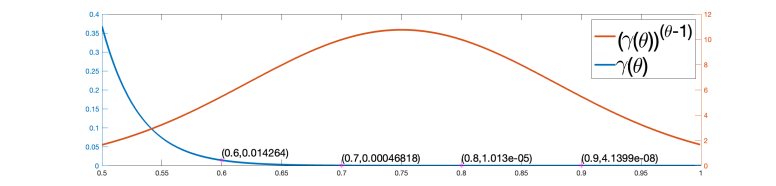
\includegraphics[width=5in]{./figures/maxwell/tauplot.pdf}
\caption{形状正则性参数(即chunkiness 参数)$\gamma(\theta)$(蓝色)($\theta$
是解的正则性阶数),即内切圆半径与外接圆半径之比,见
\eqref{rho_cont},以及误差上界常数
$(\gamma(\theta))^{(\theta-1)}$(红色)。图中给出了 $\gamma(\theta)$
的一些特定值,分别为 $\theta = 0.6, 0.7, 0.8, 0.9$.}
%这里,$\gamma(\theta)$
%对于较小的 $\theta$ 可以非常小,从而展示其适应窄单元的能力。}%更多细节见假设 \hyperref[asp:polygonG1]{(G1)} 和第 \ref{rem_assum_polygon1} 节。}
\label{fig:tauplot}
\end{figure}

\begin{figure}[htp]
\centering
\begin{subfigure}{.35\textwidth}
    \includegraphics[width=1.7in]{./figures/maxwell/taufun3.pdf}
\end{subfigure}
%%
 \begin{subfigure}{.35\textwidth}
     \includegraphics[width=1.7in]{./figures/maxwell/rho2.pdf}
\end{subfigure}
     \caption{取 $\kappa_0 = -1$。左图:不同 $\kappa_1$ 下 $\gamma(\theta)$ 与
     $\theta$ 关系。右图:$\varrho(\kappa_0,\kappa_1)$ 随 $\kappa_1$ 变化情况.}
  \label{fig:taufun} 
\end{figure}

\vspace{0.1in}

\item 关于假设 \hyperref[asp:polygonG2]{(G2)},\eqref{edge_cond_eq1} 包含了短边的情况,
即当 $h_e\rightarrow 0$ 时仍然满足要求;
而 \eqref{edge_cond_eq2} 允许某些支撑边的高度收缩,
但该边本身必须具有 $\mathcal{O}(h_K)$ 量级的长度。
我们在图 \ref{fig:submesh} 的左图中展示了一个这样的单元,
其中边 $AB$ 和 $BC$ 分别满足 \eqref{edge_cond_eq1} 和 \eqref{edge_cond_eq2}。

\vspace{0.1in}

\item 每个单元 $K$ 主要位于 $\Omega^-$ 或 $\Omega^+$,仅有一小部分可能在
    $\Omega^{\Gamma}_{\epsilon}$ 内,但 $\mathcal{B}_K$(见假设
    \hyperref[asp:polygonG3]{(G3)})可能会跨越界面 $\Gamma$。因此,我们需要定理
    \ref{thm_extension} 中的延拓算子,以便可以考虑光滑函数 $\mathcal{E}^{\pm} \bu$
    在 $\mathcal{B}_K$ 上的投影。延拓的有界性确保了估计仅依赖于
    $\|\bu\|_{\theta,\Omega^{\pm}} = \|\bu\|_{\theta,\Omega^{+}}  +
    \|\bu\|_{\theta,\Omega^{-}}$。

\end{itemize}

\end{remark}


\section{虚单元方法}
\label{sec:vspace}

在本节中,我们给出所需的 $H^1$ 和 $\bH(\rot)$
协调
虚单元空间、时谐 Maxwell 方程的虚单元方法
以及本文使用的基本估计。

\subsection{虚单元方法}
使用 \cite{BeiraoBrezziCangianiManziniEtAl2013,2016VeigaBrezziMarini} 中提出的最低阶 
$H^1$ 和 $\bH(\rot)$ 协调虚单元空间:
\begin{subequations}
\label{ive_space}
\begin{align}
&   \widetilde{V}^n_h(K) = \{ v_h \in H^1_0(K):  \nabla v_h\in \bH(\ddiv^0; K), ~ v_h|_{\partial K} \in C^1(\partial K), ~ v_h|_e \in \mathbb{P}_1(e) ~ \forall e\in \mathcal{E}_K \}, \label{ive_space1} \\
&   \widetilde{\bfV}^e_h(K) = \{ \bv_h \in \bH_0(\rot;K) \cap \bH(\ddiv^0;K):  \rot \bv_h \in \mathbb{P}_0(K), ~ (\bv_h\cdot\bt)|_e \in \mathbb{P}_0(e) ~ \forall e\in \mathcal{E}_K \}, \label{ive_space2}
\end{align}
\end{subequations}
两个空间的自由度分别是多边形顶点函数值和边上切向分量的积分。
由于局部 PDE
的稳定性与单元几何密切相关,这种定义不适合各向异性分析。因此,我们将采用
\cite{2021CaoChenGuo}
中的等价定义,该定义可以用于辅助各向异性分析。该定义使用了假设
\ref{assump_vmesh} 中定义的 “虚拟网格” 。\cite{2021CaoChenGuo}
中的空间定义如下:
\begin{subequations}
\label{auxi_v_space_1_polygon}
\begin{align}
V^n_h(K) & = \{ v_h \in H^1(K) : ~ v_h|_T\in\mathbb{P}_1(T) ~~ \forall T \in \mathcal{T}_K \},  \label{auxi_v_space_1_polygon1} \\
\bfV^e_h(K) & = \{ \bv_h \in \bH(\rot ;K): ~  \bv_h|_{T} \in \mathcal{ND}_h(T) ~~ \forall T\in \mathcal T_h(K),
~  \rot \bv_h \in \mathbb{P}_0(K)\}, \label{auxi_v_space_1_polygon2}
\end{align}
\end{subequations}
其中 $\mathcal{ND}_h(T) = \{\boldsymbol{a} + b(x_2, -x_1)^T : \boldsymbol{a} \in \mathbb{R}^2,
b \in \mathbb{R}\}$ 是标准的局部 N\'ed\'elec 空间。空间 $V^n_h(K)$ 
实际上就是定义在虚拟网格上的经典拉格朗日元空间。
在 \cite{2021CaoChenGuo} 中,作者已经证明了上述空间与 \eqref{ive_space} 
中的原始空间具有相同的节点和边自由度,
确保了这两种空间之间的同构性。因此投影算子的计算保持不变。
需要注意的是,这种同构目前只能为最低阶空间建立。

全局空间可以定义为
\begin{subequations}
\label{glob_space}
\begin{align}
&    V^n_h =  \{ v_h|_K \in V^n_h(K) ~~ \forall K\in \mathcal{T}_h \}  \cap H^1_0(\Omega) ,\\
& \bfV^e_h =  \{ \bv_h|_K \in \bfV^e_h(K) ~~ \forall K\in \mathcal{T}_h \}  \cap \bH_0(\rot;\Omega) .
\end{align}
\end{subequations}
对于任何 $\epsilon>0$,定义如下插值算子
\begin{subequations}
\label{interp}
\begin{align}
& I^n_h :  H^{1+\epsilon}(\Omega^{\pm}) \longrightarrow V^n_h, ~~~ I^n_hv_h(\bfx) = v_h(\bfx) ~~ \forall \bfx\in \mathcal{N}_h,  \\
& I^e_h : \bH^{1/2+\epsilon}(\rot; \Omega^{\pm}) \longrightarrow \bfV^e_h, ~~~ \int_e I^e_h \bv_h\cdot\bt \dd s = \int_e \bv_h\cdot\bt \dd s ~~ \forall e\in \mathcal{E}_h.
\end{align}
\end{subequations}
这里的 $I^e_h$ 是良定的,
根据 Sobolev 嵌入定理,$\bH^{1/2+\epsilon}(\rot; \Omega^{\pm})$ 的正则性意味着 
$\rot\bu|_{\Omega^{\pm}}\in L^p(\Omega^{\pm})$,
其中 $p>2$。
记 $Q_D$ 为 $L^2(D)$ 到 $\mathbb{P}_0(D)$ 的 $L^2$ 投影,
它将频繁用于区域 $D$。对于向量空间的投影,我们将保持相同的符号 $Q_D$ 
以简化表示。此外,我们定义 $\mathcal{T}_h$ 上的全局投影算子 $Q_h$ 对于 $K \in
\mathcal{T}_h$,$Q_h|_K = Q_K$。
可以证明对于 $\bv_h \in \bfV_h^e(K)$,$L^2$ 投影 $Q_K \bv_h$ 以及 $\rot \bv_h$ 可以仅基于自由度进行计算。

现在给出问题 \eqref{model1} 的虚单元方法:找到 $\bu_h\in \bfV^e_h$ 使得
\begin{equation}
\label{vem0}
a_h(\bu_h,\bv_h) = (\bsf,Q_h \bv_h)_{\Omega} ~~~~~ \forall \bv_h\in \bfV^e_h,
\end{equation}
其中
\begin{subequations}
\label{vem1}
\begin{align}
&   a_h(\bu_h,\bv_h) := (\alpha_h \rot\bu_h, \rot\bv_h)_{\Omega} - b_h(\bu_h,\bv_h),  \label{vem11}   \\
&   b_h(\bu_h,\bv_h) := \sum_{K\in\mathcal{T}_h} b_K(\bu_h,\bv_h),  \label{vem12}  \\
&    b_K(\bu_h,\bv_h) := (\beta_hQ_K \bu_h,Q_K \bv_h )_{K} + h ( (I-Q_K )\bu_h\cdot\bt ,  (I-Q_K )\bv_h\cdot\bt )_{\partial K}.  \label{vem13}
\end{align}
\end{subequations}

其中 $b_h(\cdot,\cdot)$ 实际上是一个内积,见如下引理:
\begin{lemma}
\label{bn_norm}
$b_h(\cdot,\cdot)$ 在 $\bfV^e_h$ 上定义了一个内积,因此 $\|\cdot\|_b$ 是一个范数。
\end{lemma}
\begin{proof}
我们只需要验证 $\|\bv_h\|_b=0$ 意味着 $\bv_h=\mathbf{ 0}$ 对于 $\bv_h \in \bfV^e_h$。事实上,我们立即有 $Q_K\bv_h = \mathbf{ 0}$ 在每个 $K$ 上,因此 $\bv_h\cdot\bt = 0$ 在 $\partial K$ 上。由于自由度,我们有 $\bv_h=\mathbf{ 0}$。
\end{proof}
因此我们可以为 $ \bv\in \bH^{s}(\rot;\Omega^{\pm})\oplus \bfV^e_h, s>1/2$ 引入以下范数:
\begin{equation}
\label{abnorm}
\| \bv \|^2_b:= b_h(\bv,\bv) ~~~~ \text{和} ~~~~\| \bv \|^2_a := \| \rot\bv \|^2_{0,\Omega} + \|\bv \|^2_b.
\end{equation}

\begin{remark}
\label{rem_stab}
尽管 $b_h$ 在 \eqref{vem11} 中被减去,但在 \eqref{vem13} 
中稳定化项仍然是必要的;从理论角度来看,需要稳定项来确保 \eqref{bh_l2_bound} 
中的范数等价性,使得 \eqref{Hdeomp1} 中的 Helmholtz 分解是良定的。
此外,沿切向的稳定对于确保插值误差最优且对各向异性单元形状鲁棒至关重要,
如引理 \ref{lem_interp_est} 所示。
%我们的稳定项 $b_h(\cdot,\cdot)$ 是可计算的,因为 $(\bv_h\cdot\bt)|_e$ 基本上是边上的自由度,并且可以写成 VEM 文献中的标准格式 \cite{2023Mascotto}:
%\begin{equation*}
%\label{rem_stab_eq0}
%( (I-Q_K )\bu_h\cdot\bt ,  (I-Q_K )\bv_h\cdot\bt )_{\partial K} = ( \text{DoF}((I-Q_K )\bu_h),\text{DoF}((I-Q_K )\bv_h) )_{\partial \Omega}.
%\end{equation*}
%这是用于边型 VEM 的最自然稳定项之一,因为它以自由度的形式显式表达 \cite{2022VeigaMascottoMeng,2016VeigaBrezziMarini,2020BeiroMascotto,BEIRAODAVEIGA2021}。其他类型的稳定项也可以考虑 \cite{2017VeigaDassiRusso,2023Mascotto}。我们观察到,这种稳定项足以获得令人满意的数值结果,而不会出现 \cite{2017VeigaDassiRusso} 中提到的弯曲现象。这一方面当然值得深入研究,但这超出了本文的范围。
\end{remark}

\subsection{逼近与稳定性}

我们首先回顾薄带引理 \cite[引理
2.1]{2010LiMelenkWohlmuthZou},它使我们能够处理假设 \ref{interf_eps} 中的不匹配区域 $\Omega^{\Gamma}_{\epsilon h^2}$:
\begin{lemma}
\label{lem_strip}
对于 $z\in H^{s}(\Omega^\pm)$,$s>1/2$,有
\begin{equation}
\label{lem_strip_eq0}
\| z \|_{0,\Omega^{\Gamma}_{\epsilon h^2}} \lesssim \sqrt{\epsilon} h \| z \|_{s,\Omega^{\pm}}.
\end{equation}
\end{lemma}

以下两个引理讨论投影和插值估计,其中隐藏的常数都与各向异性单元形状无关。
其证明放在 \ref{sec:lemmaproof} 节。
\begin{lemma}
\label{lem_Pi_est}
设 $\bu\in \bH^\theta(\Omega^{\pm})$,$\theta\in (1/2,1]$。在假设 \ref{assum_geo} 中的 \hyperref[asp:I2]{(I2)} 以及假设 \ref{interf_eps}、\ref{assump_vmesh} 和 \ref{assump_polygon} 下,有
\begin{equation}
\label{lem_Pi_est_eq0}
\sum_{K\in\mathcal{T}_h} \| \bu - Q_K \bu \|^2_{0,K} + h_K\| (I - Q_K )\bu\cdot \bt \|^2_{0,\partial K} \lesssim h^{2\theta} \| \bu \|^2_{\theta,\Omega^{\pm}}.
\end{equation}
\end{lemma}

\begin{lemma}
\label{lem_interp_est}
设 $\bu\in \bH^\theta(\Omega^{\pm})\cap \bH(\rot;\Omega^{\pm})$,$\theta\in (1/2,1]$。在假设 \ref{assum_geo} 中的 \hyperref[asp:I2]{(I2)} 以及假设 \ref{interf_eps}、\ref{assump_vmesh} 和 \ref{assump_polygon} 下,有
\begin{subequations}
\label{lem_interp_est_eq0}
\begin{align}
& \| \bu - I^e_h \bu \|_{0,\Omega}  \lesssim h^{\theta}  \| \bu \|_{\theta,\Omega^{\pm}} + h\|  \rot \bu \|_{0,\Omega} ,  \label{lem_interp_est_eq01}\\
& \| \bu - I^e_h \bu \|_{b} \lesssim h^{\theta}  \| \bu \|_{\theta,\Omega^{\pm}} + h\| \rot \bu \|_{0,\Omega}.   \label{lem_interp_est_eq02}
\end{align}
如果进一步的有 $\bu\in \bH^\theta(\rot;\Omega^{\pm})$,则
\begin{align}
& \| \rot( \bu - I^e_h \bu ) \|_{0,\Omega} \lesssim h^{\theta}  \| \rot \bu
\|_{\theta},\Omega^{\pm} .   \label{lem_interp_est_eq03}
\end{align}
\end{subequations}
\end{lemma}

在虚单元方法的分析中,一个关键部分是网格相关范数的有界性,
即同一空间在配备不同度量时的恒同算子的连续性
\begin{lemma}
\label{lem_L2stab}
在假设 \ref{assump_vmesh} 下,以下恒同算子是连续的
\begin{subequations}
\label{lem_L2stab_eq0}
\begin{align}
& (\bfV^e_h, \| \cdot \|_{a}) \xrightarrow[]{~~I~~}  (\bfV^e_h,\|\cdot\|_{0,\Omega}), \label{lem_L2stab_eq01} \\
&  ( \bH^{s}(\Omega^{\pm}) ,\|\cdot\|_{s,\Omega^{\pm}} ) \xrightarrow[]{~~I~~}  ( \bH^{s}(\Omega^{\pm}),\|\cdot\|_{b}) ~~~ \forall s\in(1/2,1]. \label{lem_L2stab_eq02}
\end{align}
\end{subequations}
\end{lemma}
\begin{proof}
对于 \eqref{lem_L2stab_eq01},根据 \cite[引理 3.4]{2021CaoChenGuo} 的论证,我们可以证明
\begin{equation}
\label{lem_Poincare_eq0}
\| \bv_h \|_{0,K} \le  \left( \frac{ \cot(\theta_{M}) C_K  }{2\min\{d_1,d_2\}} \right)^{1/2} (  h^{1/2}_{K} \|  \bv_h\cdot\bt \|_{0,\partial P} + h_{K} \| \rot\, \bv_h \|_{0,K}),
\end{equation}
其中 $C_K$ 是一个仅依赖于 $K$ 顶点数的整数%(见下面的备注 \ref{rem_CK})
,$d_1$ 和 $d_2$ 来自假设 \ref{assump_vmesh} 中的 \hyperref[asp:polygonL2]{(L2)}。将 \eqref{lem_Poincare_eq0} 应用于 $\bv_h - Q_K \bv_h$ 并利用 $Q_K$ 的有界性,可以得到 \eqref{lem_L2stab_eq01}。

接下来,对于 \eqref{lem_L2stab_eq02},给定 $\bv\in \bH^s(\Omega^{\pm})$,使用引理 \ref{lem_Pi_est} 和投影的有界性,我们有
\begin{equation}
\label{lem_L2stab_eq2}
\| \bv \|^2_b = \| Q_h \bv \|^2_{0,\Omega}  +  \sum_{K\in\mathcal{T}_h} h_K \| (I-Q_K )\bv\cdot\bt \|^2_{0,\partial K} \lesssim \| \bv \|^2_{0,\Omega} + h^{2s} \| \bv \|^2_{s,\Omega^{\pm}} .
\end{equation}
\end{proof}

%\begin{remark}
%\label{rem_CK}
%不等式 \eqref{lem_Poincare_eq0} 适用于悬点情况,
%这些节点在构造虚拟网格时被视为普通节点。
%具体来说,单元 $K$ 具有 $|\mathcal{N}_K|$ 个节点(包括悬挂节点),
%因此,该单元的三角剖分恰好包含 $|\mathcal{N}_K|-2$ 个三角形和 $|\mathcal{N}_K|-3$ 条内部边。
%通过一个较粗略的估计,我们可以得出 $C_K \leq |\mathcal{N}_K|-2$。
%因此,随着节点数量的增加,$C_K$ 可能趋于无穷大。
%这意味着,$K$ 的顶点数量需要满足 Assumption \ref{assump_vmesh} 所述的上界约束。
%\end{remark}

\begin{remark}
尽管 $b_h(\cdot,\cdot)$ 作为 $L^2$ 内积的近似,
引理 \ref{bn_norm} 仅能保证其正定性,而无法提供一个与单元形状无关的下界,
即 $\| \cdot \|_{0,\Omega} \lesssim \| \cdot
\|_b$,其中隐含常数无法保持与单元形状无关。
为了获得这种稳定的下界,需要包含 $\rot$ 项,如 \eqref{lem_L2stab_eq01} 所示。
返过来,仅使用 $L^2$ 范数来控制 $\|\cdot\|_b$ 也缺乏对单元形状的鲁棒性,
我们需要增强正则性,使用 $\|\cdot\|_{s,\Omega^{\pm}}$ 
控制,即 \eqref{lem_L2stab_eq02}。
\end{remark}

% 以下三个引理已在 \cite{2021CaoChenGuo,2021CaoChenGuoIVEM} 中出现,其中要求了较高的正则性,即 $s=1$。

\subsection{分解与嵌入}
\label{sec:decomp}

在本小节中,我们扩展了一些已有的正则分解,
以适应间断系数以及前述虚单元方法相关的内积的情况。
在构造所需的空间和算子后,我们可以建立以下交换图:
\begin{equation}
\label{DR_curl}
\left.
\begin{array}{ccccccc}
\mathbb R \xrightarrow[]{\quad} &     H^2(\Omega^{\pm})\cap H^1_0(\Omega) & \xrightarrow[]{~~\nabla~~} & \bH^1(\Omega^{\pm}) \cap \bH_0(\rot;\Omega) & \xrightarrow[]{~~\rot~~} & L^2(\Omega)  &\xrightarrow[]{\quad} 0  \\
~~~~& \quad \bigg\downarrow I^n_{h}  &  & ~~~~\bigg\downarrow I^e_{h}  &  &~~~~\bigg\downarrow Q_h \\
\mathbb R \xrightarrow[]{\quad}& V^n_{h} & \xrightarrow[]{~~\nabla~~} &
\bfV^e_{h} & \xrightarrow[]{~~\rot~~} & \mathbb{P}_0(\mathcal{T}_h)  &\xrightarrow[]{\quad} 0.
\end{array}\right.
\end{equation}
% 其中,由虚拟单元空间组成的序列是精确的。

\begin{lemma}
\label{lem_exact_seq}
\CC{
交换图 \eqref{DR_curl} 是可交换的,并且其下面一行的序列是恰当的。
}
\end{lemma}

\begin{proof}
由于 \eqref{auxi_v_space_1_polygon} 中的空间通过其自由度与 \eqref{ive_space} 中的经典空间同构,因此其论证方式与 \cite{2016VeigaBrezziMarini} 完全相同。
\end{proof}

接下来,我们引入 \textit{Hodge} 映射:
\begin{equation}
\label{hodge_map}
\mathcal{H}_{\beta}: \bfV^e_h \rightarrow \bfK(\beta;\Omega) ,~~~~\text{满足} ~~ \rot \mathcal{H}_{\beta}\bw_h = \rot \bw_h.
\end{equation}
由于 $\beta$ 为正数,\eqref{hodge_map} 是良定的,
由 \eqref{lem_embd_2} 可知,$\mathcal{H}_{\beta}\bfV^e_h \subset \bH^{\theta}(\Omega^{\pm})$。
% 我们还可以进一步证明关于 $\mathcal{H}_{\beta}$ 的以下引理。

类似于经典的 N\'ed\'elec 空间,$\bH(\rot)$ 协调虚单元空间并不具备全局 
散度为零的性质。
因此,我们需要在 $b_h(\cdot,\cdot)$ 这一内积意义下引入一个离散的散度为零条件。
这可以得到 $\bv_h\in \bfV^e_h$ 的一种特殊的离散 Helmholtz 分解:
\begin{equation}
\label{Hdeomp1}
\begin{split}
&\bv_h = \bw_h + \nabla q_h, ~~~~ \bw_h\in \bfV^e_h, ~~ q_h \in V^n_h, \\
\text{满足} ~~~& b_h( \bw_h , \nabla s_h) = 0 ~~ \forall s_h \in V^n_h.
\end{split}
\end{equation}
由 \eqref{lem_L2stab_eq01} 可得:
\begin{equation}
\label{bh_l2_bound}
\| \nabla v_h \|^2_{0,\Omega} \lesssim b_h(\nabla v_h,\nabla v_h) ~~~ \forall v_h \in V^n_h,
\end{equation}
\CC{这表明分解 \eqref{Hdeomp1} 是良定的。}
% 注意到,由于 $b_h$ 在 $\bfV^e_h$ 上是正定的,\eqref{Hdeomp1} 中的分解是良定义的。
% 传统定义离散 $\ddiv$-自由子空间的方法通常基于标准的 $L^2$ 内积 $(\cdot,\cdot)_{\Omega}$。

\begin{remark}
\label{rem_decomposition}
由于 $b_h(\cdot,\cdot) \approx (\cdot,\cdot)_{\Omega}$,因此用 $b_h(\cdot,\cdot)$ 替换标准的 $L^2$ 内积 $(\cdot,\cdot)_{\Omega}$ 是合理的。
此外,\eqref{Hdeomp1} 可重写为:
给定 $\bv_h\in \bfV^e_h$,寻找 $q_h\in V^n_h$ 使得
\begin{equation}
\label{rem_decomposition_eq1}
b_h(\nabla q_h, \nabla s_h) = b_h(\bv_h, \nabla s_h) ~~~ \forall s_h \in V^n_h,
\end{equation}
这实际上就是带有间断系数的 Poisson 方程的 VEM 形式。
%尽管虚拟空间的定义已被修改,但由于投影保持不变,此处的 VEM 仍与文献 \cite{2013BeiraodeVeigaBrezziCangiani,2014VeigaBrezziMariniRusso,2018CaoChen} 中的形式完全一致。
%因此,本工作的分析可以很容易地推广到 $H^1$ 方程,而由于其具有强迫定性,这一推广甚至更加简单。
$\Box$
\end{remark}

我们定义 $\bfV^e_h$ 中离散散度为零的子空间:
\begin{equation}
\label{dis_discrete}
\bfK_h(\beta_h;\Omega) = \{ \bw_h\in \bfV^e_h~:~ b_h( \bw_h, \nabla s_h) = 0 ~~
\forall s_h \in V^n_h \}.
\end{equation}
下述引理表明,通过 Hodge 映射可以估计 $\bfK_h(\beta_h;\Omega)$ 与 $\bfK(\beta;\Omega)$ 之间的近似误差。

\begin{lemma}
\label{lem_Hodge_est}
在 Assumption \ref{assum_geo} 中的假设 \hyperref[asp:I1]{(I1)} 以及网格假设 \ref{interf_eps} 和 \ref{assump_vmesh} 下,对于任意 $\bw_h \in \bfK_h(\beta_h;\Omega)$,
$\mathcal{H}_{\beta}\bw_h\in \bfK(\beta;\Omega)$ 满足:
\begin{subequations}
\label{lem_Hodge_est_eq0}
\begin{align}
& \|  \mathcal{H}_{\beta}\bw_h  \|_{\theta,\Omega^{\pm}} \lesssim \| \rot \bw_h \|_{0,\Omega}, \label{lem_Hodge_est_eq01}  \\
&  \| \mathcal{H}_{\beta}\bw_h - \bw_h \|_{b} \lesssim h^{\theta} \| \rot \bw_h \|_{0,\Omega},  \label{lem_Hodge_est_eq02}
\end{align}
\end{subequations}
其中 $\theta$ 来自引理 \ref{lem_embd_1}。
\end{lemma}

\begin{proof}
根据引理 \ref{lem_embd_1} 及 $\bfK(\beta;\Omega)$ 的性质,我们得出 $\mathcal{H}_{\beta}\bw_h\in \bH^{\theta}(\Omega^{\pm})$,并且:
$$
\|  \mathcal{H}_{\beta}\bw_h  \|_{\theta,\Omega^{\pm}} \lesssim \| \rot  \mathcal{H}_{\beta}\bw_h \|_{0,\Omega} + \| \ddiv \beta \mathcal{H}_{\beta}\bw_h \|_{0,\Omega} =  \| \rot \bw_h \|_{0,\Omega},
$$
其中最后一个等号利用了 \eqref{hodge_map} 的定义及散度为零的性质。

我们接下来分析 \eqref{lem_Hodge_est_eq02}。
定义:
$$
\bv_h := \bw_h - \mathcal{H}_{\beta}\bw_h = (\bw_h - I^e_h
\mathcal{H}_{\beta}\bw_h)+(I^e_h \mathcal{H}_{\beta}\bw_h -
\mathcal{H}_{\beta}\bw_h):= \bv^{(1)}_h + \bv^{(2)}_h.
$$
于是有:
\begin{equation}
\begin{split}
\label{lem_Hodge_est_eq5}
\| \bv_h \|^2_b =  \underbrace{(  \bw_h , \bv^{(1)}_h )_{b} }_{(I)} -
\underbrace{ (   \mathcal{H}_{\beta}\bw_h , \bv^{(1)}_h )_{b}}_{(II)}  +
\underbrace{ (  \bw_h - \mathcal{H}_{\beta}\bw_h , \bv^{(2)}_h )_{b} }_{(III)}.
\end{split}
\end{equation}
现在分别估计上述各项。
交换图 \eqref{DR_curl} 的可交换性意味着
\begin{equation}
\label{lem_Hodge_est_eq3}
\rot \bv^{(1)}_h = \rot( \bw_h - I^e_h\mathcal{H}_{\beta}\bw_h ) = \rot I^e_h(
\bw_h - \mathcal{H}_{\beta}\bw_h ) = Q_h \rot( \bw_h - \mathcal{H}_{\beta}\bw_h
) =0.
\end{equation}
由恰当序列可知,$\bv^{(1)}_h = \bw_h - I^e_h\mathcal{H}_{\beta}\bw_h\in
\nabla V^n_h\subset \nabla H^1_0(\Omega)$,因此 $\bw_h$ 的性质表明 $(I)$ 项为零。
对于 $(II)$ 项,再次利用 $\mathcal{H}_{\beta}\bw_h$ 的 $\beta$-散度为零性质,可得 $(\beta \mathcal{H}_{\beta}\bw_h, \bv_h^{(1)})_{\Omega}=0$,从而得到:
\begin{equation*}
\begin{split}
\label{lem_Hodge_est_eq4}
( \mathcal{H}_{\beta}\bw_h, \bv^{(1)}_h)_{b} = \sum_{K\in\mathcal{T}_h}
& \underbrace{ ( \beta_h Q_K \mathcal{H}_{\beta}\bw_h - \beta
\mathcal{H}_{\beta}\bw_h,  \bv^{(1)}_h)_{K} }_{(IIa)} \\
& +  \underbrace{ h ( (I-Q_K)\mathcal{H}_{\beta}\bw_h\cdot\bt,
(I-Q_K)\bv^{(1)}_h\cdot\bt )_{\partial K} }_{(IIb)}.
\end{split}
\end{equation*}
由引理 \ref{lem_Pi_est},引理 \ref{lem_L2stab} 中的 \eqref{lem_L2stab_eq01}
以及假设 \ref{interf_eps} 与引理 \ref{lem_strip},可以得到:
\begin{equation}
\begin{split}
\label{lem_Hodge_est_eq4_1}
\sum_{K\in\mathcal{T}_h}  (IIa) & = \sum_{K\in\mathcal{T}_h}( \beta_h Q_K \mathcal{H}_{\beta}\bw_h - \beta_h \mathcal{H}_{\beta}\bw_h,  \bv^{(1)}_h)_{K} + ( (\beta_h - \beta) \mathcal{H}_{\beta}\bw_h,  \bv^{(1)}_h)_{K} \\
& \le h^{\theta} \| \mathcal{H}_{\beta}\bw_h \|_{\theta,\Omega^{\pm}} \|
\bv^{(1)}_h \|_{0,\Omega} + h  \| \mathcal{H}_{\beta}\bw_h
\|_{\theta,\Omega^{\pm}} \| \bv^{(1)}_h \|_{0,\Omega}  \\
& \lesssim h^{\theta} \| \mathcal{H}_{\beta}\bw_h \|_{\theta,\Omega^{\pm}} \| \bv^{(1)}_h \|_b,
\end{split}
\end{equation}
其中 $\| \bv^{(1)}_h \|_{b} = \| \bv^{(1)}_h \|_a$。
$(IIb)$ 项的估计可直接由引理 \ref{lem_Pi_est} 得到:
\begin{equation}
\label{lem_Hodge_est_eq4_2}
\sum_{K\in\mathcal{T}_h}  (IIb) \lesssim h^{\theta} \| \mathcal{H}_{\beta}\bw_h
\|_{\theta,\Omega^{\pm}} \| \bv^{(1)}_h \|_b.
\end{equation}
注意到 $(III)\le \| \bv_h  \|_{b}\| \bv^{(2)}_h \|_{b}$,因此 \eqref{lem_Hodge_est_eq5} 变为:
\begin{equation}
\begin{split}
\label{lem_Hodge_est_eq6}
\| \bv_h \|^2_{b} &\lesssim h^{\theta} \| \mathcal{H}_{\beta}\bw_h \|_{\theta,\Omega^{\pm}} ( \| \bv_h \|_{b} + \| \bv^{(2)}_h \|_{b}) + \| \bv_h  \|_{b}\| \bv^{(2)}_h \|_{b} \\
& \lesssim h^{\theta} ( \| \mathcal{H}_{\beta}\bw_h \|_{\theta,\Omega^{\pm}} + \| \rot \mathcal{H}_{\beta}\bw_h \|_{0,\Omega} ) \| \bv_h \|_{b} \\
&  + h^{2\theta}\| \mathcal{H}_{\beta}\bw_h \|_{\theta,\Omega^{\pm}} ( \|
\mathcal{H}_{\beta}\bw_h \|_{\theta,\Omega^{\pm}} + \| \rot
\mathcal{H}_{\beta}\bw_h \|_{0,\Omega} ),
\end{split}
\end{equation}
其中在第二个不等式中,我们对 $\bv^{(2)}_h$ 应用了引理 \ref{lem_interp_est} 中的 \eqref{lem_interp_est_eq02}。
由 \eqref{lem_Hodge_est_eq01},\eqref{lem_Hodge_est_eq6} 可推出所需的估计结果。
\end{proof}

\section{误差估计}
\label{sec:erroreqn}

在本小节我们估计虚单元方法 \eqref{vem0} 的误差。仅凭
$\bu\in\bH^\theta(\rot;\Omega^{\pm})$
的正则性要求无法直接得到最优误差估计。
为了解决这一问题,我们对源项的正则性做出以下假设:
\begin{equation}
\label{fregularity}
\bsf \in \bH^{\theta}(\Omega^{\pm}) \cap \bH(\ddiv;\Omega) .
\end{equation}
这里强调一下,这仅仅是源项的正则性,而不是解的正则性。
通常情况下,由于间断系数和几何奇异性,源项的正则性不能直接与解的正则性相关联。

现在我们对虚单元方法进行误差分析。首先将解误差 $\bfe_h := \bu - \bu_h$ 分解为 $\bxi_h$ 和 $\beta_h$,其中
\begin{equation}
\label{err_decomp_1}
\bxi_h =  \bu - I^e_h \bu ~~~~ \text{且} ~~~~ \beta_h = I^e_h \bu - \bu_h.
\end{equation}
难点在于估计 $\beta_h$,思路是利用其在 $b_h(\cdot,\cdot)$ 内积下的离散分解:
\begin{equation}
\label{err_decomp_2}
\beta_h = \br_h + \nabla q_h, ~~~ \br_h\in \bfK_h(\beta_h;\Omega), ~~q_h\in V^n_h.
\end{equation}
因此,$\beta_h$ 的误差估计简化为估计 $\br_h$ 和 $\nabla q_h$。

为了估计 $\| \bfe_h \|_{0,\Omega}$,以下引理表明只需估计 $\|\bfe_h\|_a$。

\begin{lemma}
\label{lem_L2}
设 $\bu\in \bH^{\theta}(\rot;\Omega^{\pm})$ 且 $\bsf\in \bH^{\theta}(\Omega^{\pm})$。在假设 \ref{assum_geo} 的 \hyperref[asp:I2]{(I2)} 以及假设 \ref{interf_eps}、\ref{assump_vmesh} 和 \ref{assump_polygon} 下,有
\begin{equation}
\label{lem_L2_eq0}
\| \bfe_h \|_{0,\Omega} \lesssim h^{\theta} \| \bu \|_{\theta,\rot;\Omega^{\pm}} + \| \bfe_h \|_a .
\end{equation}
\end{lemma}

\begin{proof}
根据引理 \ref{lem_L2stab} 中的 \eqref{lem_L2stab_eq01},我们有 $\| \beta_h \|_{0,\Omega} \lesssim \| \beta_h \|_{a}$,因为 $\beta_h \in \bfV^e_h$。然后,通过引理 \ref{lem_interp_est} 和三角不等式,我们得到
\begin{equation}
\begin{split}
\label{lem_L2_eq1}
\| \bfe_ h \|_{0,\Omega}  \lesssim \| \bxi_h \|_{0,\Omega} + \| \beta_h \|_{a}
& \lesssim \| \bxi_h \|_{0,\Omega} + \| \bxi_h \|_a + \| \bfe_h \|_{a}\\
& \lesssim
h^{\theta} \| \bu \|_{\theta,\rot;\Omega^{\pm}} + \| \bfe_h \|_a.
\end{split}
\end{equation}
\end{proof}

需要注意的是,虚单元解 $\bu_h$ 在双线性形式 $a(\cdot,\cdot)$ 或
$a_h(\cdot,\cdot)$
下与真解并不一致。然而,我们可以证明这种相容性误差以最优阶收敛,如下面的引理所示。

\begin{lemma}
\label{lem_consist}
设 $\bu\in \bH^{\theta}(\rot;\Omega^{\pm})\cap \bH_0(\rot;\Omega)$ 满足 $[\alpha \rot \bu]_{\Gamma} = 0$,且 $\bsf\in \bH^{\theta}(\Omega^{\pm}) $。在假设 \ref{assum_geo} 的 \hyperref[asp:I2]{(I2)} 以及假设 \ref{interf_eps}、\ref{assump_vmesh} 和 \ref{assump_polygon} 下,有
\begin{equation}
\label{lem_consist_eq0}
a_h(\bfe_h,\bv_h) \lesssim h^{\theta}( \| \bsf \|_{\theta,\Omega^{\pm}} + \| \bu \|_{\theta,\rot;\Omega^{\pm}} ) \| \bv_h \|_{a} ~~~ \forall \bv_h \in \bfV^e_h.
\end{equation}
\end{lemma}
\begin{proof}
%证明类似于 \cite{2021CaoChenGuo} 中的定理 4.1。详细证明见 \ref{proof_lem_consist}。
注意到
\begin{equation}
\begin{split}
\label{lem_consist_eq1}
a_h(\bfe_h,\bv_h) & = a_h(\bu,\bv_h) - a_h(\bu_h,\bv_h)  \\
& = a_h(\bu,\bv_h) - (\bsf, \bv_h)_{\Omega} + (\bsf, \bv_h - Q_h \bv_h)_{\Omega}, \\
& =  \sum_{K\in\mathcal{T}_h}\underbrace{ (\alpha_h \rot \bu, \rot \bv_h)_{K} - ( \alpha \rot \bu, \rot \bv_h )_{K}}_{(I)} \\
& + \underbrace{ (\beta \bu, \bv_h)_{K} - b_K(\bu,\bv_h) }_{(II)} + \underbrace{ (  \bsf, \bv_h - Q_K \bv_h )_K }_{(III)} ,
\end{split}
\end{equation}
其中在第三个等式中,我们使用了分部积分,并且假设 $[\alpha \rot \bu]_{\Gamma} =
0$,$\bv_h$ 是 $\bH(\rot;\Omega)$ 协调的,满足
\begin{equation}
\begin{split}
(\bsf,\bv_h)_{\Omega}  = ( \brot \alpha \rot \bu, \bv_h)_{\Omega} - (\beta \bu, \bv_h)
= (  \alpha \rot \bu, \brot \bv_h)_{\Omega}  - (\beta \bu, \bv_h).
\end{split}
\end{equation}
我们首先通过应用引理 \ref{lem_strip} 来估计 $(I)$:
\begin{equation}
\begin{split}
\label{lem_consist_eq2}
\sum_{K\in\mathcal{T}_h} (I) & \le \| \rot \bu \|_{0,\Omega^{\Gamma}_{\epsilon h^2}} \| \rot\bv_h \|_{0,\Omega} \lesssim h \| \rot \bu \|_{\theta,\rot;\Omega^{\pm}} \| \bv_h \|_a.
\end{split}
\end{equation}
接下来,对于 $(II)$,通过引理 \ref{lem_L2stab} 中的式 \eqref{lem_L2stab_eq01},引理 \ref{lem_Pi_est} 和引理 \ref{lem_strip},我们得到
\begin{equation}
\begin{split}
\label{lem_consist_eq3}
\sum_{K\in\mathcal{T}_h}(II) & =  \sum_{K\in\mathcal{T}_h} [ \beta_h (\bu -   Q_K \bu ,  \bv_h)_{K} + ( \beta \bu -  \beta_h  \bu ,  \bv_h)_{K}  \\
& ~~~~~~~~~~~~ -  h_K ( (I - Q_K)\bu\cdot\bt , (I - Q_K)\bv_h\cdot\bt  )_{\partial K} ] \\
& \lesssim \| \bu \|_{0,\Omega^{\Gamma}_{\epsilon h^2}} \| \bv_h \|_{0,\Omega}  + h^{\theta} \| \bu \|_{\theta,\rot,\Omega^{\pm}} \| \bv_h \|_a  \lesssim h^{\theta} \| \bu \|_{\theta,\rot,\Omega^{\pm}} \| \bv_h \|_a  .
\end{split}
\end{equation}
至于 $(III)$,通过插入 $Q_K \bsf$ 并利用引理 \ref{lem_Pi_est} 和引理 \ref{lem_L2stab} 中的式 \eqref{lem_L2stab_eq01},我们得到
\begin{equation}
\begin{split}
\label{lem_consist_eq4}
& \sum_{K\in\mathcal{T}_h} (III)  = \sum_{K\in\mathcal{T}_h}  ( \bsf - Q_K \bsf, \bv_h - Q_K \bv_h )_K \\
\lesssim & \left(\sum_{K\in\mathcal{T}_h} \| \bsf - Q_K \bsf \|^2_{0,K} \right)^{1/2} \left( \sum_{K\in\mathcal{T}_h} \|  \bv_h - Q_K \bv_h  \|^2_{0,K} \right)^{1/2}
\lesssim h^{\theta} \| \bsf \|_{\theta,\Omega^{\pm}}  \| \bv_h  \|_a.
\end{split}
\end{equation}
将式 \eqref{lem_consist_eq2}-\eqref{lem_consist_eq4} 代入式 \eqref{lem_consist_eq1},得到所需的结果。

\end{proof}
\begin{lemma}
\label{lem_consist_a}
设 $\bu,\bv\in \bH^{\theta}(\rot;\Omega^{\pm})$ 且 $\bsf\in \bH^{\theta}(\Omega^{\pm}) $。在假设 \ref{assum_geo} 的 \hyperref[asp:I2]{(I2)} 以及假设 \ref{interf_eps}、\ref{assump_vmesh} 和 \ref{assump_polygon} 下,有
\begin{equation}
\label{lem_consist_a_eq0}
a(\bfe_h, I^e_h \bv) \lesssim h^{\theta} (  \| \bsf \|_{\theta,\Omega^{\pm}} + \| \bu_h \|_{b} ) \| \bv \|_{\theta,\rot;\Omega^{\pm}}.
\end{equation}
\end{lemma}

\begin{proof}
%类似的估计可以在 \cite{2018BrennerSung} 中找到。详细证明见附录中的 \ref{proof_lemma_consist_a}。
我们注意到
\begin{equation}
\begin{split}
\label{lem_consist_a_eq1}
a(\bfe_h, \bv_h ) & = \underbrace{( (\alpha \rot \bu, \rot I^e_h\bv)_{\Omega}  - (\beta \bu, I^e_h\bv)_{\Omega} )}_{(I)} \\
&  - \underbrace{ ( (\alpha \rot \bu_h, \rot I^e_h\bv)_{\Omega}  - b_h(\bu_h, I^e_h\bv) ) }_{(II)}  - \underbrace{ ( b_h(\bu_h, I^e_h\bv) - (\beta  \bu_h, I^e_h\bv )_{\Omega}) }_{(III)}.
\end{split}
\end{equation}
根据 \eqref{vem0},我们可以得到
\begin{equation}
\begin{split}
\label{lem_consist_a_eq2}
(II) & = (\alpha_h \rot \bu_h, \rot I^e_h\bv )_{\Omega}  - b_h(\bu_h, I^e_h\bv) + ( (\alpha-\alpha_h) \rot \bu_h, \rot I^e_h\bv)_{\Omega} \\
& = (\bsf, Q_h I^e_h\bv )_{\Omega} + ( (\alpha-\alpha_h) \rot \bu_h, \rot \bv)_{\Omega}  + ( (\alpha-\alpha_h) \rot \bu_h, \rot (I^e_h\bv - \bv) )_{\Omega}.
\end{split}
\end{equation}
由于 $(I) = (\bsf, I^e_h\bv)_{\Omega}$,通过类似于 \eqref{lem_consist_eq1} 中 $(III)$ 的论证,结合引理 \ref{lem_interp_est_eq03} 和引理 \ref{lem_strip} 中的薄带论证,我们得到
\begin{equation}
\begin{split}
\label{lem_consist_a_eq3}
(I) - (II)  = & (\bsf , I^e_h\bv - Q_h I^e_h\bv)_{\Omega}  -  ( (\alpha-\alpha_h) \rot \bu_h, \rot \bv)_{\Omega}  - ( (\alpha-\alpha_h) \rot \bu_h, \rot (I^e_h\bv - \bv) )_{\Omega} \\
\lesssim &  h^{\theta}  \| \bsf \|_{\theta,\Omega^{\pm}} \|  I^e_h\bv \|_{a} +  h^{\theta}  \| \rot \bu_h \|_{0,\Omega} \| \rot\bv \|_{\theta,\Omega^{\pm}} .
\end{split}
\end{equation}
此外,结合引理 \ref{lem_interp_est},可以得到 $\| I^e_h \bv \|_a \lesssim \| \bv \|_{\theta,\rot;\Omega^{\pm}}$。
接下来,考虑 \eqref{lem_consist_a_eq1} 中的 $(III)$,我们注意到
\begin{equation}
\begin{split}
\label{lem_consist_a_eq4}
(III) = & \underbrace{ (\beta_h  \bu_h, Q_h I^e_h \bv - I^e_h \bv)_{\Omega} }_{(IIIa)} + \underbrace{ ( (\beta_h - \beta)\bu_h, I^e_h \bv - \bv )_{\Omega} }_{(IIIb)}\\
& + \underbrace{ ( (\beta_h - \beta)\bu_h,  \bv )_{\Omega} }_{(IIIc)} - \underbrace{ h \sum_{K\in\mathcal{T}_h} ( (I-Q_K)\bu_h\cdot\bt, (I-Q_K) I^e_h\bv\cdot\bt)_{\partial K} }_{(IIId)} .
\end{split}
\end{equation}
对于 $(IIIa)$ 的估计,我们结合 \eqref{lem_interp_est_eq01} 和引理 \ref{lem_Pi_est},得到
\begin{equation}
\label{lem_consist_a_eq5}
\| Q_h I^e_h \bv - I^e_h \bv \|_{0,\Omega} \le \| Q_h(I^e_h\bv-\bv) \|_{0,\Omega} + \| Q_h \bv - \bv \|_{0,\Omega}
+ \| \bv - I^e_h \bv \|_{0,\Omega}  \lesssim h^{\theta} \| \bv \|_{\theta,\rot;\Omega^{\pm}}.
\end{equation}
$(IIIb)$ 可以直接从 \eqref{lem_interp_est_eq01} 中得到估计,而 $(IIIc)$ 可以通过引理 \ref{lem_strip} 中的薄带论证进行估计。
接下来,我们估计 $(IIId)$。\CC{使用 Hölder 不等式}、\eqref{lem_interp_est_eq02} 和引理 \ref{lem_Pi_est},我们得到
\begin{equation}
\label{lem_consist_a_eq6}
(IIId) \lesssim \| \bu_h \|_b \left(( \| I^e_h \bv - \bv \|_b +  h \sum_{K\in\mathcal{T}_h} \|(I - Q_K)\bv\cdot\bt \|^2_{0,\partial K}  \right)
\lesssim h^{\theta} \| \bu_h \|_b \| \bv \|_{\theta,\rot;\Omega^{\pm}}.
\end{equation}
将上述估计合并到 \eqref{lem_consist_a_eq4} 中,我们得到 $(III)$ 的估计。结合 \eqref{lem_consist_a_eq3},我们得到了所需的估计。
\end{proof}

现在,我们准备估计 $\|\bfe_h\|_{b}$ 和 $\| \rot\bfe_h \|_{0,\Omega}$,从而得到 $\| \bfe_h \|_a$ 的估计。这是通过推广 \cite{2009ZhongShuWittumXu} 中的论证来实现的。

\begin{lemma}
\label{lem_err0}
设 $\bu\in \bH^{\theta}(\rot;\Omega^{\pm})\cap \bH_0(\rot;\Omega)$ 满足 $[\alpha \rot \bu]_{\Gamma} = 0$,且 $\bsf\in \bH^{\theta}(\Omega^{\pm}) $。在假设 \ref{assum_geo} 的 \hyperref[asp:I2]{(I2)} 以及假设 \ref{interf_eps}、\ref{assump_vmesh} 和 \ref{assump_polygon} 下,有
\begin{equation}
\label{lem_err0_eq0}
\| \bfe_h \|_{b} \lesssim h^{\theta} ( \| \bsf \|_{\theta,\Omega^{\pm}} + \| \bu \|_{\theta,\rot,\Omega^{\pm}})  +  \| \br_h \|_b.
\end{equation}
\end{lemma}

\begin{proof}
应用 H\"older 不等式可以得到
\begin{equation}
\begin{split}
\label{lem_err0_eq1}
b_h(\bfe_h,\bfe_h) & = b_h(\bfe_h, \bxi_h) +  b_h(\bfe_h, \br_h) +  b_h(\bfe_h, \nabla q_h) \\
& \leqslant \| \bxi_h \|^2_b + \| \br_h \|^2_b + \| \bfe_h \|^2_b/2 + |b_h(\bfe_h, \nabla q_h) |.
\end{split}
\end{equation}
$\bxi_h$ 的估计已由引理 \ref{lem_interp_est} 中的 \eqref{lem_interp_est_eq02} 给出。我们只需估计 \eqref{lem_err0_eq1} 右边的最后一项。根据引理 \ref{lem_consist},由于 $|a_h(\bfe_h,\nabla q_h)| = |b_h(\bfe_h,\nabla q_h)|$,我们有
\begin{equation}
\begin{split}
\label{lem_err0_eq2}
|b_h(\bfe_h, \nabla q_h)| &\lesssim h^{\theta}
(\| \bsf \|_{\theta,\Omega^{\pm}} + \| \bu \|_{\theta,\rot,\Omega^{\pm}})
\| \nabla q_h \|_b \\
& \le  h^{2\theta}  (\| \bsf \|_{\theta,\Omega^{\pm}}+
\| \bu \|_{\theta,\rot,\Omega^{\pm}})^2
+ ( \| \bfe_h \|^2_b + \| \bxi_h \|^2_b + \| \br_h \|^2_b)/4.
\end{split}
\end{equation}
将 \eqref{lem_err0_eq2} 代入 \eqref{lem_err0_eq1},我们得到所需的估计。
\end{proof}

\begin{lemma}
\label{lem_errcurl}
设 $\bu\in \bH^{\theta}(\rot;\Omega^{\pm})\cap \bH_0(\rot;\Omega)$ 满足 $[\alpha \rot \bu]_{\Gamma} = 0$,且 $\bsf\in \bH^{\theta}(\Omega^{\pm}) $。在假设 \ref{assum_geo} 的 \hyperref[asp:I2]{(I2)} 以及假设 \ref{interf_eps}、\ref{assump_vmesh} 和 \ref{assump_polygon} 下,有
\begin{equation}
\label{lem_errcurl_eq0}
\| \rot \bfe_h \|_{0,\Omega} \lesssim h^{\theta} ( \| \bsf \|_{\theta,\Omega^{\pm}} + \| \bu \|_{\theta,\rot,\Omega^{\pm}})   +  \| \br_h \|_b.
\end{equation}
\end{lemma}
\begin{proof}
由 \eqref{err_decomp_2} 可知:
\begin{equation}
\begin{split}
\label{lem_errcurl_eq1}
\| \alpha^{1/2}_h \rot \bfe_h \|^2_0 &= a_h(\bfe_h,\bfe_h) + \| \bfe_h \|^2_{b}  = a_h(\bfe_h, \bxi_h) + a_h(\bfe_h,\beta_h) + b_h(\bfe_h,\bxi_h+\beta_h) \\
& = (\alpha_h \rot \bfe_h, \rot \bxi_h)_{\Omega} +  a_h(\bfe_h,\beta_h)  + b_h(\bfe_h,\br_h)  + b_h(\bfe_h, \nabla q_h).
\end{split}
\end{equation}
引理 \ref{lem_consist} 和 $|a_h(\bfe_h,\bxi_h)| = |b_h(\bfe_h,\bxi_h)|$ 给出
\begin{subequations}
\label{lem_errcurl_eq2}
\begin{align}
&  a_h(\bfe_h,\beta_h) \lesssim  h^{\theta}
(\| \bsf \|_{\theta,\Omega^{\pm}}+ \| \bu \|_{\theta,\rot,\Omega^{\pm}})
( \| \rot \bfe_h \|_{0,\Omega} + \| \bfe_h \|_{b} + \| \bxi_h \|_{a} ). \\
&  |b_h(\bfe_h, \nabla q_h)| \lesssim  h^{\theta}
(\| \bsf \|_{\theta,\Omega^{\pm}} + \| \bu \|_{\theta,\rot,\Omega^{\pm}})
( \| \bfe_h \|_b + \| \bxi_h \|_b + \| \br_h \|_b  ).
\end{align}
\end{subequations}
此外,$b_h(\bfe_h,\br_h) \le \| \bfe_h \|_b \| \br_h \|_b$。将此估计和 \eqref{lem_errcurl_eq2} 代入 \eqref{lem_errcurl_eq1},应用类似于 \eqref{lem_err0_eq2} 的论证,并使用引理 \ref{lem_err0},我们得到 \eqref{lem_errcurl_eq0}。
\end{proof}

现在,基于引理 \ref{lem_errcurl} 和 \ref{lem_err0},我们只需估计 $\br_h$。

\begin{lemma}
\label{lem_rh}
设 $\bu\in \bH^{\theta}(\rot;\Omega^{\pm})\cap \bH_0(\rot;\Omega)$ 满足 $[\alpha \rot \bu]_{\Gamma} = 0$,且 $\bsf\in \bH^{\theta}(\Omega^{\pm})$。在假设 \ref{assum_geo}-\ref{assump_polygon} 下,假设 $h$ 足够小,使得 $h < h_{\star}$,其中 $h_{\star}$ 在下面的证明中定义,则有
\begin{equation}
\label{lem_rh_eq0}
\| \br_h \|_b  \lesssim h^{\theta}  ( \| \bsf \|_{\theta,\Omega^{\pm}} + \| \bu \|_{\theta,\rot,\Omega^{\pm}}).
\end{equation}
\end{lemma}

\begin{proof}
我们考虑 \eqref{hodge_map} 中定义的 Hodge 映射。由于 $\br_h\in \bfK_h(\beta;\Omega)$,根据引理 \ref{lem_interp_est} 中的 \eqref{lem_interp_est_eq03},并使用引理 \ref{lem_Hodge_est} 和 \ref{lem_errcurl},我们有
\begin{equation}
\begin{aligned}
\label{lem_rh_eq1}
\| \br_h - \mathcal{H}_{\beta} \br_h \|_{b} \lesssim h^{\theta} \| \rot \br_h \|_{0,\Omega}
& \leq  h^{\theta} \left( \| \rot \bfe_h \|_{0,\Omega} + \| \rot \bxi_h \|_{0,\Omega}  \right) \\
& \lesssim  h^{2\theta}  (\| \bsf \|_{\theta,\Omega^{\pm}} + \| \bu \|_{\theta,\rot,\Omega^{\pm}})
+   h^{\theta}  \| \br_h \|_b  .
\end{aligned}
\end{equation}
因此,存在常数 $C$ 使得
\begin{equation}
\label{lem_rh_eq2}
(1 - C h^{\theta})\| \br_h \|_b \lesssim h^{2\theta}  \| \bsf \|_{\theta,\Omega^{\pm}}   + \| \mathcal{H}_{\beta} \br_h \|_{b}.
\end{equation}
设 $h_{\star}$ 为满足 $1 - C h_{\star}^{\theta} = 0$ 的阈值。我们现在使用对偶论证来估计 $\| \mathcal{H}_{\beta} \br_h \|_{b}$。考虑以下 $\bw \in \bH_0(\rot;\Omega)\cap\bH(\beta,\ddiv;\Omega)$ 的辅助问题:
\begin{equation}
\label{lem_rh_eq3}
\brot \alpha \rot \bw - \beta \bw = \beta \mathcal{H}_{\beta} \br_h.
\end{equation}
由于该问题与模型问题具有相同的系数,以下稳定性成立:
\begin{equation}
\label{lem_rh_eq3_1}
\| \bw \|_{\theta,\rot,\Omega^{\pm}} \lesssim \| \mathcal{H}_{\beta} \br_h \|_{0,\Omega}.
\end{equation}
将 \eqref{lem_rh_eq3} 两端同时与 $\bv\in\bH_0(\rot;\Omega)$ 做 $L^2$ 内积,有
\begin{equation}
\label{lem_rh_eq4}
a(\bw,\bv) = (\alpha\rot \bw, \rot \bv)_{\Omega} - (\beta \bw, \bv)_{\Omega} = (\beta \mathcal{H}_{\beta} \br_h,\bv)_{\Omega}.
\end{equation}
由于 $\mathcal{H}_{\beta} \br_h\subset\bfK(\beta;\Omega)$,如 \eqref{div_free} 所示,有
\begin{equation}
\label{lem_rh_eq5}
a(\bw,\nabla q) = -(\beta \bw, \nabla q)_{\Omega} = 0 ~~~ \forall q \in H^1_0(\Omega).
\end{equation}
由于 $\rot(\mathcal{H}_{\beta} \br_h) = \rot(\br_h) =
\rot(\beta_h)$,根据恰当复形,$\mathcal{H}_{\beta} \br_h -\beta_h \in \nabla H^1_0(\Omega)$。因此,\eqref{lem_rh_eq5} 表明
\begin{equation}
\label{lem_rh_eq6}
a(\bw,\mathcal{H}_{\beta} \br_h -\beta_h) = - (\beta \bw, \mathcal{H}_{\beta} \br_h -\beta_h)_{\Omega} = 0.
\end{equation}
此外,在 \eqref{lem_rh_eq4} 中取 $\bv =\mathcal{H}_{\beta} \br_h$,并利用 \eqref{lem_rh_eq6} 可得
\begin{equation}
\begin{split}
\label{lem_rh_eq7}
\| \sqrt{\beta} \mathcal{H}_{\beta} \br_h \|^2_{0,\Omega} & = a(\bw, \mathcal{H}_{\beta} \br_h) = a(\bw, \mathcal{H}_{\beta} \br_h - \beta_h) + a(\bw, \beta_h) \\
& = a(\bw - I^e_h \bw, \bfe_h ) + a(I^e_h \bw, \bfe_h ) - a(\bw, \bxi_h) := (I) + (II) + (III).
\end{split}
\end{equation}
我们接下来对各项进行估计。
对于 $(I)$,引理 \ref{lem_interp_est} 中的 \eqref{lem_interp_est_eq01} 和 \eqref{lem_interp_est_eq03} 可得
\begin{equation}
\label{lem_rh_eq8}
(I) \lesssim \| \bfe_h \|_{a}  \| \bw - I^e_h \bw \|_{a} \lesssim h^{\theta} \|
\bw \|_{\theta,\rot;\Omega^{\pm}}  \| \bfe_h \|_{a}.
\end{equation}
$(II)$ 项的估计可由引理 \ref{lem_consist_a} 得到,而 $(III)$ 则可再次利用引理 \ref{lem_interp_est} 进行估计。
将这些估计代入 \eqref{lem_rh_eq7},利用 \eqref{lem_rh_eq3_1} 并消去 \eqref{lem_rh_eq7} 中的 $\|\mathcal{H}_{\beta}\br_h\|_{0,\Omega}$,可得
\begin{equation}
\begin{split}
\label{lem_rh_eq10}
\|  \mathcal{H}_{\beta} \br_h \|_{0,\Omega}
\lesssim h^{\theta} ( \| \bsf \|_{\theta;\Omega^{\pm}}
+ \| \bu \|_{\theta,\rot;\Omega^{\pm}}
+  \| \bu_h \|_{b}  + \| \bfe_h \|_{a}  ).
\end{split}
\end{equation}
此外,由 $\| \bu_h \|_b \le \| \bfe_h \|_b + \| \bu \|_b$,可知 $\| \bu \|_b$ 的估计可由引理 \ref{lem_L2stab} 中的 \eqref{lem_L2stab_eq02} 得到。
然后利用引理 \ref{lem_err0} 和 \ref{lem_errcurl} 估计 $\| \bfe_h\|_a \lesssim \| \bfe_h \|_{b} + \| \rot \bfe_h \|_{0,\Omega}$。
因此,\eqref{lem_rh_eq10} 可推出 $\| \mathcal{H}_{\beta} \br_h \|_{0,\Omega}  \lesssim h^{\theta} ( \| \bsf \|_{\theta;\Omega^{\pm}} + \| \br_h \|_b )$。
结合引理 \ref{lem_L2stab} 中的 \eqref{lem_L2stab_eq02} 以及引理
\ref{lem_Hodge_est} 中的 \eqref{lem_Hodge_est_eq01},最终可得
\begin{equation}
\begin{split}
\label{lem_rh_eq11}
\|  \mathcal{H}_{\beta} \br_h \|_{b} & \lesssim \| \mathcal{H}_{\beta} \br_h
\|_{0,\Omega} + h^{\theta} \| \rot \br_h \|_{0,\Omega}  \\
& \lesssim h^{\theta} (
\| \bsf \|_{\theta;\Omega^{\pm}} + \| \bu \|_{\theta,\rot;\Omega^{\pm}} + \| \br_h \|_b + \| \rot \br_h \|_{0,\Omega} ) \\
& \lesssim h^{\theta} ( \| \bsf \|_{\theta;\Omega^{\pm}} + \| \bu \|_{\theta,\rot;\Omega^{\pm}}+ \| \br_h \|_b + \| \rot \bfe_h \|_{0,\Omega} +
\| \rot \bxi_h \|_{0,\Omega} )   \\
& \lesssim h^{\theta} ( \| \bsf \|_{\theta;\Omega^{\pm}} + \| \bu \|_{\theta,\rot;\Omega^{\pm}}+ \| \br_h \|_b )。
\end{split}
\end{equation}
不等式中我们也使用了引理 \ref{lem_errcurl} 和 \eqref{lem_interp_est_eq03}。
将 \eqref{lem_rh_eq11} 代入 \eqref{lem_rh_eq2},
假设 $h$ 足够小,使得 $h<h_{\star}$,且满足 $1-Ch^{\theta}>0$,
利用 $h^{\theta}\lesssim 1$,我们得到所需的 $\| \br_h \|_b$ 估计。
\end{proof}

最后,通过上述估计,我们可以得到以下定理中的最优误差估计。

\begin{theorem}
\label{lem_error}
设 $\bu \in \bH^{\theta}(\rot;\Omega^{\pm}) \cap \bH_0(\rot;\Omega)$,满足 $[\alpha \rot \bu]_{\Gamma} = 0$,
并且 $\bsf \in \bH^{\theta}(\Omega^{\pm})$。
在假设 \ref{assum_geo}-\ref{assump_polygon} 下,
假设 $h$ 足够小,使得 $h < h_{\star}$($h_{\star}$ 在引理 \ref{lem_rh} 中给出),
且 $\beta$ 不是特征值,
那么存在唯一的 $\bu_h$ 满足 \eqref{vem0},并且有
\begin{equation}
\label{lem_error_eq0}
\| \bfe_h \|_{\rot;\Omega} \lesssim h^{\theta} ( \| \bsf \|_{\theta,\Omega^{\pm}} + \| \bu \|_{\theta,\rot,\Omega^{\pm}}).
\end{equation}
\end{theorem}

\begin{proof}
应用引理 \ref{lem_rh} 到引理 \ref{lem_err0} 和 \ref{lem_errcurl},得到
$\| \bfe_h\|_a \lesssim h^{\theta} ( \| \bsf \|_{\theta,\Omega^{\pm}} + \| \bu \|_{\theta,\rot,\Omega^{\pm}})$。
然后,使用引理 \ref{lem_L2},我们有
$\| \bfe_h\|_{0,\Omega} \lesssim h^{\theta} ( \| \bsf \|_{\theta,\Omega^{\pm}} + \| \bu \|_{\theta,\rot,\Omega^{\pm}})$。
因此 \eqref{lem_error_eq0} 成立。
现在证明离散问题 \eqref{vem0} 的适定性。
令 $\bsf=0$,因为 $\beta$ 不是特征值所以连续问题适定,
所以 $\bu=0$。因此,根据 \eqref{lem_error_eq0} 可得 $\bu_h=0$,证明完成。
\end{proof}

%\begin{remark}
%注意,$h_{\star} = C^{-1/\theta}$ 来自 \eqref{lem_rh_eq2}。
%虽然常数 $C$ 可能依赖于 $\beta$,
%但它与网格大小 $h$ 和网格正则性无关。
%\end{remark}
\section{引理 \ref{lem_Pi_est} 和 \ref{lem_interp_est} 的证明}
\label{sec:lemmaproof}

在本节中,我们将基于第 \ref{sec:mesh_assump} 节中的几何假设验证引理
\ref{lem_Pi_est} 和 \ref{lem_interp_est}。以下的 Poincar\'e
\cite[引理 7.1]{2017ErnGuermond} 不等式将在证明中频繁使用。
\begin{lemma}
\label{lem_proj_approxi}
设 \( D \) 为一个开域,对于所有 \( v \in H^s(D) \) 且 \( s \in (0,1) \),有
\begin{align}
\label{lem_proj_approxi_eq01}
\| v - Q_D v \|_{L^2(D)} \le h^{s+1}_D |D|^{-1/2} |v|_{s,D}.
\end{align}
\end{lemma}
另一个有用的结果是关于不规则单元上的分数阶 Sobolev 范数的不等式。
\begin{lemma}
\label{lem_geometry_patch}
设 \( S \) 为一边长为 \( h \) 的正方形,\( \widetilde{S} \) 为其矩形子区域,其中一边与 \( S \) 的边重合,且相应的支撑高度为 \( l \)。那么,对于任意 \( u \in H^s(S) \),\( s > 1/2 \),有
\begin{equation}
\label{lem_geometry_patch_eq0}
\int_{\widetilde{S}} \int_{\widetilde{S}} (u(\bfa) - u(\bfb) )^2 \, \dd \bfa \, \dd \bfb \le h^2 l^{2s}  |u |^2_{s,S}.
\end{equation}
\end{lemma}
\begin{proof}
%参见附录 \ref{sec:proof_lem_geometry_patch} 中的证明。

设 $\bfa=(a_1,a_2)$ 和 $\bfb=(b_1,b_2)$。
不失一般性,我们构造一个坐标系,使得 $S$ 和 $\widetilde{S}$ 的公共边为 $x_1$ 轴,垂直边为 $x_2$ 轴。然后,我们有
\begin{equation}
\begin{split}
\label{lem_geometry_patch_eq1}
\int_{\widetilde{S}} \int_{\widetilde{S}} (u(\bfa) - u(\bfb) )^2 \dd \bfa \dd \bfb & = \int_0^l \int_0^l \int_0^h \int_0^h (u(a_1,a_2) - u(b_1,b_2) )^2  \dd a_1 \dd b_1 \dd a_2 \dd b_2 \\
& \lesssim \underbrace{ \int_0^l \int_0^l \int_0^h \int_0^h (u(a_1,a_2) - u(a_1,b_2) )^2  \dd a_1 \dd b_1  \dd a_2 \dd b_2}_{(I)} \\
& + \underbrace{ \int_0^l \int_0^l \int_0^h \int_0^h (u(a_1, b_2) - u(b_1,b_2) )^2  \dd a_1 \dd b_1 \dd a_2 \dd b_2 }_{(II)}.
\end{split}
\end{equation}
令 $e_{a_1}$ 为垂直于边 $e$ 的边,$x_1$ 坐标为 $a_1$。我们知道 $u \in H^{s-1/2}(e_{a_1})$,因此
\begin{equation}
\begin{split}
\label{lem_geometry_patch_eq2}
(I) & = h \int_0^h \int_0^l \int_0^l  (u(a_1,a_2) - u(a_1,b_2) )^2 \dd a_2 \dd b_2  \dd a_1  \\
& \le h l^{2s}  \int_0^h \int_0^l \int_0^l  (u(a_1,a_2) - u(a_1,b_2) )^2/ |a_2-b_2|^{1+2(s-1/2)} \dd a_2 \dd b_2  \dd a_1 \\
& \le h l^{2s} \int_0^h |u(a_1,\cdot)|^2_{s-1/2,e_{a_1}} \dd a_1 \le h^2 l^{2s}  |u |^2_{s,S},
\end{split}
\end{equation}
其中我们使用了分数阶 Sobolev 正常定义和到 $S$ 的迹不等式,假设 $S$ 是形状正则的。
至于 $(II)$,我们使用类似的论证:
\begin{equation}
\begin{split}
\label{lem_geometry_patch_eq3}
(II) &= l \int_0^l  \int_0^h \int_0^h (u(a_1, b_2) - u(b_1,b_2) )^2  \dd a_1 \dd b_1  \dd b_2 \\
& \le l h^{2s} \int_0^l  \int_0^h \int_0^h (u(a_1, b_2) - u(b_1,b_2) )^2/ |a_1 - b_2|^{1+2(s-1/2)}  \dd a_1 \dd b_1  \dd b_2 \le l^2 h^{2s}  |u |^2_{s,S}.
\end{split}
\end{equation}
结合 \eqref{lem_geometry_patch_eq1} 和 \eqref{lem_geometry_patch_eq2} 得到所需结果。
\end{proof}

我们回顾 \cite{stein1970singular,2015Zhou} 中关于带有 Lipschitz 域的分数 Sobolev 空间扩展的定理。
\begin{theorem}
\label{thm_extension}
对于任意满足 \eqref{Dregular} 的区域 \( D \),存在一个连续的扩展算子
$$
\mathcal{E}_D : H^s(D) \longrightarrow H^s(\mathbb{R}^2) .
$$
\end{theorem}
利用此定理和假设 \ref{assum_geo} 中的 \hyperref[asp:I2]{(I2)},
我们可以通过设定
$ D = \Omega^{\pm} $ 构造 $ \mathcal{E}^{\pm}:=\mathcal{E}_{\Omega^{\pm}}$。
为了简化表达,对于任意与
$ \Gamma $ 相交的域 $ D \subseteq \Omega $,我们引入
\begin{equation}
\label{Enorm}
\| \bu \|_{E,s,D} := \|\mathcal{E}^+ \bu^+ \|_{s,D} + \| \mathcal{E}^- \bu^- \|_{s,D}.
\end{equation}
根据 $ \mathcal{E}^{\pm} $ 的有界性,我们有
\begin{equation}
\label{Enorm2}
\| \bu \|_{E,s,\Omega} \lesssim \| \bu \|_{s,\Omega}.
\end{equation}
上式中的常数只依赖于 $\Gamma$ 和 $\Omega^{\pm}$,
而不依赖于网格。

下面我们忽略靠近界面的非常薄的区域,在这些区域上 $ \alpha_h $ 和 $ \beta_h $
可能与 $ \alpha $ 和 $ \beta $ 不同,如图 \ref{fig:interfelem}
所示。我们可以通过假设 \ref{interf_eps} 和引理 \ref{lem_strip}
中给出的薄带引理来有效地处理这个问题。为了简化起见,以下分析中我们将不考虑这一问题。

\subsection{引理 \ref{lem_Pi_est} 的证明}
\label{subsec:lem_Pi_est}
由于假设 \hyperref[asp:polygonG3]{(G3)} 所规定的有限重叠性质以及定理
\ref{thm_extension} 给出的连续扩展,我们只需要在每个单元 \( K \)
上局部进行估计,并结合 \( \| \bu \|_{E,\theta,\mathcal{B}_K} \)
来完成证明。为了简化讨论,假设 \( K \subseteq \Omega^+ \)。显然,\(
\mathcal{B}_K \) 可能会穿过 \( \Gamma \) 且不完全包含在 \( \Omega^{+} \)
中,这正是我们引入 \( \mathcal{E}^{\pm}\bu^{\pm} \) 的原因。

对于 \eqref{lem_Pi_est_eq0} 中的第一项,我们使用引理 \ref{lem_proj_approxi} 立即得到
\begin{equation}
\label{verify_lem_Pi_est_polygon_eq1}
\| \bu - Q_K \bu \|_{0,K} \le \| \bu^+ - Q_{\mathcal{B}_K} \mathcal{E}^+ \bu^+ \|_{0,K}
\lesssim \|  \mathcal{E}^+ \bu^+ - Q_{\mathcal{B}_K} \mathcal{E}^+ \bu^+ \|_{0,\mathcal{B}_K}
\lesssim h^{\theta}_K |  \mathcal{E}^+ \bu |_{\theta,\mathcal{B}_K}.
\end{equation}
对于 \eqref{lem_Pi_est_eq0} 中的第二项,我们分别讨论满足 \eqref{edge_cond_eq1} 或 \eqref{edge_cond_eq2} 的边 \( e \) 的两种情况。对于 \eqref{edge_cond_eq1} 的情况,首先进行如下分解:
\begin{equation}
\label{verify_lem_Pi_est_polygon_eq2}
\| (I - Q_K)\bu \cdot \bt \|_{0,e} \le \| (\bu^+ - Q_{\mathcal{B}_K} \mathcal{E}^+ \bu^+ ) \cdot \bt \|_{0,e}
+ \| (Q_{\mathcal{B}_K} \mathcal{E}^+ \bu^+  - Q_K\bu^+) \cdot \bt \|_{0,e}.
\end{equation}
由于 \( e \) 可以看作是 \( \mathcal{B}_K \)
中某个形状正则的三角形的一部分,上式右侧的第一项可以利用引理 7.2
中的迹不等式进行估计。接下来我们聚焦于第二项,使用 \eqref{edge_cond_eq1}
进一步推导
\begin{equation}
\begin{split}
\label{verify_lem_Pi_est_polygon_eq2_1}
&\| (Q_{\mathcal{B}_K} \mathcal{E}^+ \bu^+  - Q_K\bu^+) \cdot \bt \|_{0,e}  \le h_e^{1/2} | Q_{\mathcal{B}_K} \mathcal{E}^+ \bu^+  - Q_K\bu^+ | \\
= & h_e^{1/2} |K|^{-1} |\int_K Q_{\mathcal{B}_K} \mathcal{E}^+ \bu^+  -
\bu^+ \, \dd \bfx | \\
\le & h_e^{1/2}|K|^{-1/2}\| Q_{\mathcal{B}_K} \mathcal{E}^+ \bu  - \bu \|_{0,K}
\le 6 \sqrt{c_1/\pi} h^{\theta-1/2}_K | \mathcal{E}^+ \bu |_{\theta,\mathcal{B}_K}.
\end{split}
\end{equation}

难点在于情况 \eqref{edge_cond_eq2},由于支撑高度可能收缩,即
$$
h_K h_e |K|^{-1} \le c_2 \, h_K/l_e \rightarrow \infty,
$$
因此不能简单地应用 \eqref{verify_lem_Pi_est_polygon_eq2_1} 中的论证。这里,我们采用完全不同的思路。
考虑一条具有最大长度的边 $e_K$,且我们知道 $|e_K|\simeq h_K$。令 $l_K$ 为 $e_K$ 在 $K$ 内的支撑高度。我们构造一个正方形 $\mathcal{S}_K\subseteq \mathcal{B}_K$,同时满足 $\mathcal{S}_K\supseteq K$,使得其有一边(记作 $\bar{e}$)与 $e_K$ 重合,且长度为 $\mathcal{O}(h_K)$。为简便起见,我们可以假设 $\mathcal{S}_K$ 就是边长为 $h_K$ 的正方形;否则,只需略微调整其尺寸。几何示意请参见图 \ref{fig:block}。
对于每个 $e\in\mathcal{E}_K$,在整个正方形 $\mathcal{S}_K$ 上的迹不等式给出
\begin{equation}
\label{verify_lem_Pi_est_polygon_eq3}
\| (I - Q_K)\bu \cdot \bt \|_{0,e} \lesssim h^{-1/2}_K \| \mathcal{E}^+ \bu^+ - Q_{K} \mathcal{E}^+ \bu^+ \|_{0,\mathcal{S}_K}.
\end{equation}

接下来,我们对 \eqref{verify_lem_Pi_est_polygon_eq3} 右侧进行估计。
引入局部坐标系 $(x_1,x_2)$,其中 $x_1$ 与 $\bar{e}$ 平行,并令 $e(b_2)$ 表示平行于 $\bar{e}$ 的线段,其 $x_2$ 坐标为 $b_2\in (0,l_K)$。因此,$K$ 实际上包含在一个高度为 $l_K$ 的矩形中,记作 $\widetilde{\mathcal{S}}_K$,如图 \ref{fig:block} 所示。为了简化记号,下面将 $Q_{e(b_2)}$ 简记为 $Q_{b_2}$。

利用投影算子 $Q_{K}$、$Q_{\mathcal{S}_K}$ 和 $Q_{b_2}$,应用三角不等式得到
\begin{equation}
\begin{split}
\label{verify_lem_Pi_est_polygon_eq4}
\| \mathcal{E}^+ \bu^+ - Q_{K} \mathcal{E}^+ \bu^+ \|^2_{0,\mathcal{S}_K}
&\lesssim \underbrace{\| \mathcal{E}^+ \bu^+ - Q_{\mathcal{S}_K} \mathcal{E}^+ \bu^+ \|^2_{0,\mathcal{S}_K}}_{(I)} \\
&\quad + \underbrace{\| Q_{\mathcal{S}_K} \mathcal{E}^+ \bu^+ - Q_{b_2} \mathcal{E}^+ \bu^+ \|^2_{0,\mathcal{S}_K}}_{(II)} \\
&\quad + \underbrace{\| Q_{b_2} \mathcal{E}^+ \bu^+ - Q_{K} \mathcal{E}^+ \bu^+ \|^2_{0,\mathcal{S}_K}}_{(III)}.
\end{split}
\end{equation}
对 $(I)$ 的估计可直接由引理 \ref{lem_proj_approxi} 得出。
对于 $(II)$,利用投影性质、 Hölder 不等式、迹不等式以及引理 \ref{lem_proj_approxi},有
\begin{equation}
\begin{split}
\label{verify_lem_Pi_est_polygon_eq5}
(II) &= |\mathcal{S}_K|\, |e(b_2)|^{-2} \left|\int_{e(b_2)} \Bigl(Q_{\mathcal{S}_K} \mathcal{E}^+ \bu^+ - \mathcal{E}^+ \bu^+\Bigr) \, \dd \bfx \right|^2 \\
&\le |\mathcal{S}_K|\, |e(b_2)|^{-1} \| Q_{\mathcal{S}_K} \mathcal{E}^+ \bu^+ - \mathcal{E}^+ \bu^+ \|^2_{0,e(b_2)} \\
&\lesssim \| Q_{\mathcal{S}_K} \mathcal{E}^+ \bu^+ - \mathcal{E}^+ \bu^+ \|^2_{0,\mathcal{S}_K}
\lesssim h^{2\theta}_K \, | \mathcal{E}^+ \bu^+ |^2_{\theta,\mathcal{S}_K}.
\end{split}
\end{equation}
最难处理的是 $(III)$。通过类似于 \eqref{verify_lem_Pi_est_polygon_eq5} 的推导,可以将 $(III)$ 改写为
\begin{equation}
\begin{split}
\label{verify_lem_Pi_est_polygon_eq6}
(III) &= |\mathcal{S}_K|\, |K|^{-2} \left|\int_{K} \Bigl(Q_{b_2} \mathcal{E}^+ \bu^+ - \mathcal{E}^+ \bu^+\Bigr) \, \dd \bfx \right|^2\\
&\le |\mathcal{S}_K|\, |K|^{-1} \| \mathcal{E}^+ \bu^+ - Q_{b_2} \mathcal{E}^+ \bu^+ \|^2_{0,\widetilde{\mathcal{S}}_K}.
\end{split}
\end{equation}

%注意到 $|\mathcal{S}_K|\, |K|^{-1}$ 可能会由于 $K$ 收缩而趋于无穷,
%因此需要更细致的分析。
对 \eqref{verify_lem_Pi_est_polygon_eq6} 中的 $(III)$ 关于 $b_2$ 从 $0$ 到 $l_K$ 积分,并利用 $Q_{b_2}$ 的定义以及 Hölder 不等式得到
{\small
\begin{equation}
\begin{split}
\label{verify_lem_Pi_est_polygon_eq7}
\int_0^{l_K} & (III)\, \dd b_2 \le |\mathcal{S}_K|\, |K|^{-1} \int_0^{l_K} \int_0^{l_K} \int_0^{h_K} \Bigl( \mathcal{E}^+ \bu^+(a_1,a_2) - Q_{b_2} \mathcal{E}^+ \bu^+ \Bigr)^2 \dd a_1 \dd a_2 \dd b_2 \\
&\le |\mathcal{S}_K|\, |K|^{-1} \int_0^{l_K} \int_0^{l_K} \int_0^{h_K} h_K^{-2} \left( \int_0^{h_K} \Bigl(\mathcal{E}^+ \bu^+(a_1,a_2) - \mathcal{E}^+ \bu^+(b_1,b_2)\Bigr) \dd b_1 \right)^2 \dd a_1 \dd a_2 \dd b_2 \\
&\le |\mathcal{S}_K|\, |K|^{-1} h_K^{-1} \int_0^{l_K} \int_0^{l_K} \int_0^{h_K} \int_0^{h_K} \Bigl(\mathcal{E}^+ \bu^+(a_1,a_2) - \mathcal{E}^+ \bu^+(b_1,b_2)\Bigr)^2 \dd b_1 \dd a_1 \dd a_2 \dd b_2 \\
&\le |\mathcal{S}_K|\, |K|^{-1} \, h_K\, l_K^{2\theta} \, | \mathcal{E}^+ \bu |^2_{\theta,\mathcal{S}_K}
\le c^2_2 \, h_K^2\, l_K^{2\theta-1} \, | \mathcal{E}^+ \bu^+ |^2_{\theta,\mathcal{S}_K},
\end{split}
\end{equation}
}
其中在最后一步中我们使用了引理 \ref{lem_geometry_patch} 和 \eqref{edge_cond_eq2}。

现在,对 \eqref{verify_lem_Pi_est_polygon_eq4} 中的 $\| \mathcal{E}^+ \bu^+ - Q_{K} \mathcal{E}^+ \bu^+ \|^2_{0,\mathcal{S}_K}$ 关于 $b_2$ 从 $0$ 到 $l_K$ 积分,将 $(I)$ 至 $(III)$ 的估计代入,并注意到其与 $b_2$ 无关,我们得到
\begin{equation}
\label{verify_lem_Pi_est_polygon_eq8}
\| \mathcal{E}^+ \bu^+ - Q_{K} \mathcal{E}^+ \bu^+ \|^2_{0,\mathcal{S}_K}
\lesssim h_K^{2\theta} \, | \mathcal{E}^+ \bu^+ |^2_{\theta,\mathcal{S}_K}
+ h_K^2\, l_K^{2\theta-2} \, | \mathcal{E}^+ \bu^+ |^2_{\theta,\mathcal{S}_K}.
\end{equation}
接着,应用假设 \hyperref[asp:polygonG1]{(G1)} 中的 \eqref{rho_cont},因为
$l_K\ge\rho_K$ 且 $\theta\in(1/2,1]$,根据 \eqref{maxvc},我们得到
\begin{equation}
\label{verify_lem_Pi_est_polygon_eq9}
h_K^2\, l_K^{2\theta-2} = h_K^{2\theta} \left(\frac{h_K}{l_K}\right)^{2(1-\theta)}
\le h_K^{2\theta} \, (\gamma(\theta))^{2(\theta-1)}
\le h_K^{2\theta} \, (\varrho(\kappa_0,\kappa_1))^2.
\end{equation}
将 \eqref{verify_lem_Pi_est_polygon_eq9} 代入 \eqref{verify_lem_Pi_est_polygon_eq8} 以及 \eqref{verify_lem_Pi_est_polygon_eq3},选择 $\kappa_0 = 0.5$ 和 $\kappa_1 = 60$(其他选择及其对估计的影响见 Remark \ref{rem_assum_polygon1}),我们得到
\begin{equation}
\label{verify_lem_Pi_est_polygon_eq10}
h_K^{1/2} \| (I - Q_K)\bu \cdot \bt \|_{0,e}
\lesssim c_2 \, h_K^{\theta} \, | \mathcal{E}^+ \bu^+ |_{\theta,\mathcal{B}_K},
\end{equation}
这便得到了与 \eqref{verify_lem_Pi_est_polygon_eq1} 对应的所需局部估计。全局估计则由假设 \hyperref[asp:polygonG3]{(G3)} 所施加的有限重叠性得出。

\begin{figure}[h]
\centering
\includegraphics[width=2.5in]{./figures/maxwell/block4}
\caption{单元 $K$ 及辅助正方形 $\mathcal{S}_K$ 的示意图。$K$ 包含在一个高度为
$l_K$ 的矩形 $\widetilde{\mathcal{S}}_K$ 内。$e(b_2)$ 是一段平行于 $x_1$
轴(即沿 $\bar{e}$ 方向)的线段.}
\label{fig:block}
\end{figure}

\subsection{引理 \ref{lem_interp_est} 的证明}
类似地,我们只需在每个单元上局部进行估计即可。
最简单的是 \eqref{lem_interp_est_eq03},可以根据交换图 \eqref{DR_curl} 得出,
其中投影的逼近性质由引理 \ref{lem_proj_approxi} 给出。

对于 \eqref{lem_interp_est_eq01},使用三角不等式得到
\begin{equation}
\label{verify_lem_interp_est_eq2}
\| \bxi_h  \|_{0,K} \le \| \bu - Q_K \bu \|_{0,K} + \| Q_K \bu - I^e_h \bu \|_{0,K}.
\end{equation}
右边第一项的估计来自于引理 \ref{lem_Pi_est}。
对于第二项,由于 $Q_K \bu - I^e_h \bu \in \bfV^e_h(K)$ 对于所有的 $K \in \mathcal{T}_h$,应用引理 \ref{lem_L2stab} 中的 \eqref{lem_Poincare_eq0} 以及三角不等式得到
\begin{equation}
\begin{split}
\label{verify_lem_interp_est_eq3}
\| Q_K \bu - I^e_h \bu \|_{0,K} %& \lesssim h_K \| \rot I^e_h \bu \|_{0,K} + h^{1/2}_K \|  (Q_h \bu - I^e_h \bu)\cdot\bt \|_{0,\partial K} \\
\lesssim h_K \| \rot I^e_h \bu \|_{0,K} +  h^{1/2}_K \|  (Q_K \bu - \bu)\cdot\bt \|_{0,\partial K} +  h^{1/2}_K \|  ( \bu - I^e_h \bu)\cdot\bt \|_{0,\partial K}.
\end{split}
\end{equation}
接下来,右侧第一项的估计直接来自于 \eqref{lem_interp_est_eq03},
第二项的估计则由引理 \ref{lem_Pi_est} 得到。现在我们集中讨论 \eqref{verify_lem_interp_est_eq3} 右侧的第三项。

对于每个边 $e\in\mathcal{E}_K$,假设 $e \subseteq \Omega^+$,并且不失一般性,假设存在一个边 $\tilde{e} \subseteq \mathcal{B}_K$,其长度为 $\mathcal{O}(h_K)$。
然后,利用投影性质、引理 7.2 中的迹不等式 \cite{2017ErnGuermond} 以及引理 \ref{lem_proj_approxi},我们得到
\begin{equation}
\begin{split}
\label{verify_lem_interp_est_eq12}
\| ( \bu - I^e_h \bu)\cdot\bt \|_{0,e} & = \| \bu\cdot\bt - Q_e (\bu\cdot\bt) \|_{0,e} \\
& \le \| (\mathcal{E}^+\bu^+)\cdot\bt - (Q_{\mathcal{B}_K} \mathcal{E}^+\bu^+)\cdot\bt \|_{0,\tilde{e}} \\
& \lesssim h^{-1/2}_K \| \mathcal{E}^+\bu^+ - Q_{\mathcal{B}_K} \mathcal{E}^+\bu^+ \|_{0,\mathcal{B}_K}
+ h^{\theta-1/2}_K | \mathcal{E}^+\bu^+ |_{\theta,\mathcal{B}_K} \\
& \lesssim h^{\theta-1/2}_K | \mathcal{E}^+\bu^+ |_{\theta,\mathcal{B}_K}.
\end{split}
\end{equation}
因此,\eqref{lem_interp_est_eq01} 可以结合假设
\hyperref[asp:polygonG3]{(G3)},
通过将这些估计代入 \eqref{verify_lem_interp_est_eq3} 来完成。

接下来,对于 \eqref{lem_interp_est_eq02},通过三角不等式并对 $Q_K\bxi_h$ 应用 \eqref{lem_Poincare_eq0},我们得到
\begin{equation}
\begin{split}
\label{verify_lem_interp_est_eq4}
\|  \bxi_h \|^2_{b} %& \lesssim \| Q_K \bxi_h \|^2_{0,\Omega} +  h \sum_{K\in\mathcal{T}_i} ( \| Q_K \bxi_h\cdot\bt \|^2_{0,\partial K} + \| \bxi_h\cdot\bt \|^2_{0,\partial K} ) \\
\lesssim h \sum_{K\in\mathcal{T}_i} ( \| Q_K \bxi_h\cdot\bt \|^2_{0,\partial K} + \| \bxi_h\cdot\bt \|^2_{0,\partial K} ).
\end{split}
\end{equation}
这里,$\| \bxi_h\cdot\bt \|^2_{0,\partial K}$ 的估计与 \eqref{verify_lem_interp_est_eq12} 相同。
下面估计 $\| Q_K \bxi_h\cdot\bt \|_{0,\partial K}$。

我们依然根据 \eqref{edge_cond} 将讨论分为两种情况。
对于一个边 $e \in \mathcal{E}_K$,我们首先考虑 \eqref{edge_cond_eq1}。
由于 $Q_K\bxi_h$ 在 $K$ 上是常向量,我们有
\begin{equation}
\label{verify_lem_interp_est_polygon_eq1}
\| Q_K \bxi_h \cdot\bt \|_{0,e} =  h_e^{1/2}|K|^{-1} \left|\int_K \bxi_h
\cdot\bt \dd \bfx\right| \le \sqrt{c_1} h^{-1/2}_K \| \bxi_h \|_{0,K},
\end{equation}
其估计由上述 \eqref{lem_interp_est_eq01} 给出。
现在假设 $e$ 满足 \eqref{edge_cond_eq2},
由于单元 $K$ 可能极其收缩,因此 \eqref{verify_lem_interp_est_polygon_eq1} 中的论证不再适用。
不失一般性,我们可以让 $e$ 沿 $x_1$ 轴,故 $\bt_e = [1,0]^\top$。
构造 $p^e_h = x_2 \in \mathbb{P}_1(K)$ 使得 $\brot p^e_h = \bt_e$。
然后,利用投影性质和分部积分,我们得到
\begin{equation}
\begin{split}
\label{verify_lem_interp_est_polygon_eq5}
\| Q_K\bxi_h\cdot\bt_e \|_{0,e}& = h^{1/2}_e |K|^{-1} |\int_K \bxi_h\cdot
\brot p^e_h \dd \bfx  | \\
& \le \underbrace{ h^{1/2}_e |K|^{-1} \| \rot \bxi_h \|_{0,K} \| p^e_h \|_{0,K} }_{(I)} +  \underbrace{ h^{1/2}_e |K|^{-1} \| \bxi_h \cdot \bt \|_{0,\partial K}  \|  p^e_h \|_{0,\partial K} }_{(II)}.
\end{split}
\end{equation}
注意到 $ \| p^e_h \|_{\infty,K} \le l_e$,我们结合 \eqref{edge_cond_eq2} 以及
\eqref{verify_lem_interp_est_eq12} 和 \eqref{lem_interp_est_eq03} 可以得到
\begin{subequations}
\label{verify_lem_interp_est_polygon_eq6}
\begin{align}
(I) & \le h^{1/2}_e |K|^{-1/2} l_e  \| \rot \bxi_h \|_{0,K} \le \sqrt{c_2} l^{1/2}_e \| \rot \bu \|_{0,K} \lesssim \sqrt{c_2}  h^{1/2}_K \| \rot \bu \|_{0,K}, \\
(II) & \le h^{1/2}_e |K|^{-1} |\partial K|^{1/2} l_e \| \bxi_h \cdot \bt \|_{0,\partial K}  \lesssim c_2 h_K^{1/2} h^{-1/2}_e |  \mathcal{E}^+  \bu^+ |_{\theta,\mathcal{B}_K}
\lesssim c^{3/2}_2  h^{\theta-1/2}_K |  \mathcal{E}^+  \bu^+ |_{\theta,\mathcal{B}_K}.
\end{align}
\end{subequations}
最后,通过将 \eqref{verify_lem_interp_est_polygon_eq6} 代入 \eqref{verify_lem_interp_est_polygon_eq5},我们完成了证明。

%\section{引理 \ref{lem_consist} 的证明}
%\label{proof_lem_consist}
%
%\section{引理 \ref{lem_consist_a} 的证明}
%\label{proof_lemma_consist_a}
%
%
%\section{引理 \ref{lem_geometry_patch} 的证明}
%\label{sec:proof_lem_geometry_patch}

\section{数值算例}
\begin{figure}[h]
\centering
\begin{subfigure}{.48\textwidth}
\centering
\includegraphics[width=1.2in]{./figures/maxwell/convergence_test.pdf}
\end{subfigure}
\begin{subfigure}{.48\textwidth}
\centering
\includegraphics[width=1.2in]{./figures/maxwell/quadmesh.pdf}
\end{subfigure}
\caption{左图:算例 \ref{subsec:examp1},网格大小 $h = 1/16$;右图:算例
\ref{subsec:examp2},网格大小 $h = 1/16$.}
\label{fig:example12}
\end{figure}

本节将通过数值实验验证所提出方法的有效性。前两个算例旨在验证方法在界面几何形状、
解的正则性和网格单元形状正则性方面的收敛性和鲁棒性;
第三个算例中,我们探讨了误差相对于参数 $\beta$ 的关系;
第四个算例考虑了具有几何奇异性的两种复杂界面形状;
在最后一个算例中,我们将该方法应用于极薄层问题。
最后两个算例均涉及较大的波数。
所有网格均由直接切割背景笛卡尔网格得到。本节的代码均基于 FEALPy 
软件库实现 \cite{fealpy}.

\subsection{收敛阶}
\label{subsec:examp1}
设区域和界面几何为
$$
\Omega = (-1, 1)\times(-1, 1), \quad \Omega^- = \{(x, y): x^2+y^2 < \left(\frac{\pi}{5}\right)^2\}, \quad \Omega^+ = \Omega\setminus\Omega^-,
$$
如图 \ref{fig:example12} 左图所示。取参数
$$
\alpha|_{\Omega^-} = \beta|_{\Omega^-} = 1,\quad \alpha|_{\Omega^+} = \beta|_{\Omega^+} = 10,
$$
并设真解为
$$
{\bf u} = \left\{
\begin{aligned}
& - k_0(r_0^2 - x^2 - y^2)
\begin{pmatrix}
y\\
x
\end{pmatrix} \quad& \text{ in } \Omega^-, \\
& -\frac{1}{10} \, k_1(r_0^2 - x^2 - y^2)(r_1^2 - x^2 - y^2)
\begin{pmatrix}
y\\
x
\end{pmatrix} \quad& \text{ in } \Omega^+,
\end{aligned}
\right.
$$
其中 $r_0 = \frac{\pi}{5}$, $r_1 = 1$, $k_1 = 20$, $k_0 = k_1(r_1^2 - r_0^2)$.
数值结果见表 \ref{tab:exm0}。从表中可以看出,
$$
\|\bu - Q_h \bu_h\|_{0,\Omega} = O(h),\quad \|\rot \bu - \rot\bu_h\|_{0,\Omega} = O(h),
$$
这显然是最优的。

\begin{table}[!htp]
\centering
\caption{算例 \ref{subsec:examp1} 中误差 $\|\bu - Q_h \bu_h\|_{0,\Omega}$ 与
$\|\rot \bu - \rot \bu_h\|_{0,\Omega}$.}
\label{tab:exm0}
\begin{tabular}[c]{|c|c|c|c|c|c|}
\hline
$h$ & $1/8$ & $1/16$ & $1/32$ & $1/64$ & $1/128$ \\\hline
$\| {\bf u} - Q_h{\bf u}_h \|_{0,\Omega}$ & 4.798e-01 & 2.192e-01 & 1.007e-01 & 4.761e-02 & 2.303e-02 \\\hline
阶数 & -- & 1.13 & 1.12 & 1.08 & 1.05 \\\hline
$\|\rot {\bf u} - \rot {\bf u}_h\|_{0,\Omega}$ & 1.155e+00 & 5.722e-01 & 2.726e-01 & 1.366e-01 & 6.846e-02 \\\hline
阶数 & -- & 1.01 & 1.07 & 1.00 & 1.00 \\\hline
\end{tabular}
\end{table}

\subsection{对单元形状的鲁棒性}
\label{subsec:examp2}

仍然考虑区域
$\Omega=(-1, 1)\times(-1, 1)$,但界面为
$\Gamma = \{(x, y): x=\varepsilon, -1<y<1\}$,如图 \ref{fig:example12} 右图所示。
真解和参数如下所示:
$$
\bu =
\begin{pmatrix}
|x-\varepsilon|^{\theta-\frac{1}{2}} + \cos(x + y) \\
\sin(x + y)
\end{pmatrix}, \quad \alpha = 1, \quad
\beta|_{\Omega^-} = 1, \quad \beta|_{\Omega^+} = 2,
$$
其中 $\Omega^- = \{(x, y): x > \varepsilon\}, \Omega^+ = \Omega - \Omega^-$,且 $\theta > \frac{1}{2}$。
在此情况下,解 $\bu$ 属于 $\bH^{\theta}(\Omega)$。
我们设置 $\varepsilon = 1e-7$ 和 $h = 2^{-k}, k = 3, 4, 5, 6,
7$,因此在界面附近会生成非常小的单元。
不同 $\theta$ 值的数值结果见表 \ref{tab:error1} 和
\ref{tab:error2},这些结果表明了 
$\|\bu - Q_h \bu_h\|_{0,\Omega} = O(h^{\theta})$ 这达到了最优收敛率。
另外,因为网格中一些单元不仅具有短边,而且随着 $\epsilon \rightarrow 0$,
其内切球会逐渐缩小,因此数值结果还表明,
虚单元方法对各向异性的单元形状具有很强的鲁棒性;

\begin{table}[!h]
\centering
\caption{在 $\theta=0.7$ 时,算例 \ref{subsec:examp2} 中的误差 $\|\bu - Q_h
\bu_h\|_{0,\Omega}$ 和 $\|\rot \bu - \rot \bu_h\|_{0,\Omega}$.}
\label{tab:error1}
\begin{tabular}[c]{|c|c|c|c|c|c|c|}\hline
$h$ & $1/8$ & $1/16$ & $1/32$ & $1/64$ & $1/128$
\\\hline
$\| \bu - Q_h\bu_h\|_{0,\Omega}$ & 4.428e-01 & 2.729e-01 & 1.681e-01 & 1.036e-01 & 6.381e-02
\\\hline
收敛阶数 & -- & 0.7  & 0.7  & 0.7  & 0.7
\\\hline
$\|\rot {\bf u} - \rot {\bf u}_h\|_{0,\Omega}$ & 2.138e-01 & 1.037e-01 & 5.136e-02 & 2.559e-02 & 1.277e-02
\\\hline
收敛阶数 & -- & 1.04 & 1.01 & 1.   & 1.
\\\hline
\end{tabular}
\end{table}

\begin{table}[!h]
\centering
\caption{在 $\theta=0.51$ 时,算例 \ref{subsec:examp2} 中的误差 $\|\bu - Q_h
\bu_h\|_{0,\Omega}$ 和 $\|\rot \bu - \rot \bu_h\|_{0,\Omega}$.}
\label{tab:error2}
\begin{tabular}[c]{|c|c|c|c|c|c|}\hline
自由度 (Dof) &   161 &   577 &  2177 &  8449 & 33281
\\\hline
$\| \bu - Q_h\bu_h\|_{0,\Omega}$ & 8.264e-01 & 5.818e-01 & 4.091e-01 & 2.875e-01 & 2.019e-01
\\\hline
收敛阶数 & -- & 0.51 & 0.51 & 0.51 & 0.51
\\\hline
$\|\rot {\bf u} - \rot {\bf u}_h\|_{0,\Omega}$ & 2.258e-01 & 1.078e-01 & 5.301e-02 & 2.630e-02 & 1.310e-02
\\\hline
收敛阶数 & -- & 1.07 & 1.03 & 1.01 & 1.01
\\\hline
\end{tabular}
\end{table}

\subsection{对 $\beta$ 的影响}
\label{subsec:exampwave}

误差界中的常数 $\|\bu - Q_h \bu_h\|_{0,\Omega} \leq Ch$ 和
$\|\rot \bu - \rot \bu_h\|_{0,\Omega} \leq Ch$ 与 $h$ 无关,
但可能与 $\beta$ 有关。
在本算例中,我们通过考察相对误差
$$
\frac{\|\bu - Q_h \bu_h\|_{0,\Omega}}{h\|\bu\|_{0,\Omega}},
\quad
\frac{\|\rot \bu - \rot \bu_h\|_{0,\Omega}}{h\|\bu\|_{0,\Omega}}.
$$
来研究虚单元方法对 $\beta$ 的鲁棒性。
采用与算例 \ref{subsec:examp2} 相同的定义域和界面设置,并且
$\varepsilon = 0$,我们考虑参数 $\alpha = 1, \beta|_{\Omega^+} = 1$。
真解为
$$
\mathbf{u} = \left\{
\begin{aligned}
\begin{pmatrix}
2\cos(ax)\cos(cy) \\
2\sin(ax)\sin(cy)
\end{pmatrix} \quad &\text{ in } \Omega^{+} 中, \\
\begin{pmatrix}
\cos(bx)\cos(cy) \\
\sin(bx)\sin(cy)
\end{pmatrix} \quad &\text{ in } \Omega^{-} 中.
\end{aligned}
\right.,
$$
其中 $a = \sqrt{1/2}, b = \sqrt{\beta^-/2}, c = b-2a$。
使用网格大小 $h = 1/2^{10}$ 和不同的 $\beta^-$ 值的数值结果如图
\ref{fig:beta_convergence} 所示,结果表明
$$
\frac{\|\bu - Q_h \bu_h\|_{0,\Omega}}{h\|\bu\|_{0,\Omega}} = O((\beta^-)^{1/2}),
\quad
\frac{\|\rot \bu - \rot \bu_h\|_{0,\Omega}}{h\|\bu\|_{0,\Omega}} =
O(\beta^-).
$$
\begin{figure}[h]
\centering
\includegraphics[width=3in]{./figures/maxwell/error_with_different_beta.pdf}
\caption{算例 \ref{subsec:exampwave} 中 VEM 对 $\beta^-$ 的相对误差.}
\label{fig:beta_convergence} %% label for first subfigure
\end{figure}

\subsection{几何奇异性}
\label{subsec:geo_sing}
在这个例子中,我们考虑了两种具有几何奇异性的界面:
第一种由两个圆形区域的交集形成,导致两个尖点;
第二种是由多边形界面形成的尖点。设
$\Omega=(0, 4)\times(0, 1)$,$\Omega^+ = \Omega - \Omega^-$,并且
\begin{figure}[h]
\centering
\includegraphics[width=4in]{./figures/maxwell/mesh_double_circle.pdf}
\caption{ 算例 \ref{subsec:geo_sing} 中界面 1 的几何形状.}
\label{fig:interfacedoublecircle}
\end{figure}
\begin{figure}[h]
\centering
\includegraphics[width=4in]{./figures/maxwell/poly_interface.pdf}
\caption{算例 \ref{subsec:geo_sing} 中界面 2 的几何形状.}
\label{fig:interfacepoly}
\end{figure}
$$
\Omega^- = \left\{
\begin{aligned}
&\{(x, y) : (x-1.75)^2 + y^2 < r^2  \text{ or }
(x-1.25)^2 + y^2 < r^2  \},\quad
& \text{ 界面 1,}\\
&\mathrm{Polygon}
\left\{
\begin{matrix}
& (3.117, 0.500),
& (2.906, 0.523),
& (2.250, 0.320),\\
& (2.062, 0.807),
& (1.980, 0.333),
& (1.781, 0.847),\\
& (1.753, 0.377),
& (1.003, 0.312),
& (2.438, 0.177),\\
& (2.875, 0.477).
& &
\end{matrix}
\right\}
& \text{ 界面 2.}\\
\end{aligned}
\right.,
$$
其中 $r = 0.35$,见图 \ref{fig:interfacedoublecircle} 以获取示意图。
设源项、参数和边界条件为
$$
\alpha = 1, \quad \beta = \omega^2 \left( \epsilon + {\rm i} \frac{\sigma}{\omega} \right), \quad {\bf f} = -{\rm i}\omega \begin{pmatrix}
0\\
1
\end{pmatrix} \exp\left(-\frac{(x-3)^2}{\epsilon^2}\right), \quad g = 0.
$$
其中 ${\rm i} = \sqrt{-1}$,$\sigma|_{\Omega^-} = 1$,$\sigma|_{\Omega^+} = 0.1$。
注意,在此情况下,$\beta$ 包含虚部,这使得问题是正定的。

由于在此情形下构造解析解较为困难,
我们将使用在网格大小为 $h = 1/2^8$ 时计算出的解作为参考解,记作 $\bu^8_h$。
对于界面 1,$\omega = 100$, $\epsilon = 0.5$ 的情况,
数值结果如表 \ref{tab:exm3-0} 所示,这表明了最优的收敛性。
同时,需要指出,当网格加密后,收敛率变得略微超线性。
我们认为这种现象可能是由于参考解并非真解,而仅仅是细网格上的数值解。

同时,对于大波数的情况,我们比较了 VEM 和经典 FEM 在网格大小 $h = 1/2^{10}$ 时的数值解,
结果如图 \ref{fig:femvsvemdoublecircle}(界面 1 )和图
\ref{fig:femvsvempoly}(界面 2 )所示,
可以看到结果是相似的。

\begin{table}[!h]
\centering
\caption{算例 \ref{subsec:geo_sing} 中类型 1 界面,$\epsilon = 0.5$,$\omega =
5$ 时的解误差.}
\label{tab:exm3-0}
\begin{tabular}[c]{|c|c|c|c|c|c|}\hline
$k$ & $3$ & $4$ & $5$ & $6$ & $7$
\\\hline
$\|Q_h{\bf u}_h^8 - Q_h{\bf u}_h^k\|_{0,\Omega}$ & 6.234e-02 & 2.644e-02 & 1.234e-02 & 5.915e-03 & 2.634e-03
\\\hline
阶数 & -- & 1.24 & 1.1  & 1.06 & 1.17
\\\hline
$\|{\rm rot} {\bf u}_h^8 - {\rm rot} {\bf u}_h^k\|_{0,\Omega}$  & 2.223e-01 & 9.508e-02 & 4.455e-02 & 2.138e-02 & 9.521e-03
\\\hline
阶数 & -- & 1.23 & 1.09 & 1.06 & 1.17
\\\hline
\end{tabular}
\label{tab:eps05}
\end{table}

\begin{table}[!htp]
\centering
\caption{算例 \ref{subsec:geo_sing} 中类型 1 界面,$\epsilon = 0.01$,$\omega =
100$ 时的解误差.}
\label{tab:exm3-2}
\begin{tabular}[c]{|c|c|c|c|c|c|c|c|}\hline
$k$ & $3$ & $4$ & $5$ & $6$ & $7$
\\\hline
$\| Q_h\bu_h^8 - Q_h\bu_h^k\|_{0,\Omega}$ & 7.961e-02 & 3.619e-02 & 1.228e-02 & 5.072e-03 & 2.125e-03
\\\hline
阶数 & -- & 1.14 & 1.56 & 1.28 & 1.25
\\\hline
$\|\rot \bu_h^8 - \rot \bu_h^k\|_{0,\Omega}$ & 8.554e-01 & 3.945e-01 & 1.530e-01 & 7.135e-02 & 3.066e-02
\\\hline
阶数 & -- &  1.12 &  1.37 &  1.1  &  1.22
\\\hline
\end{tabular}
\end{table}

\begin{figure}[!h]
\centering
\includegraphics[width=5in]{./figures/maxwell/two_circle.pdf}
\caption{类型 1 界面的 FEM(左)与 VEM(右)比较,网格大小为 $h = 1/2^{10}$.}
\label{fig:femvsvemdoublecircle}
\end{figure}

\begin{figure}[!h]
\centering
\includegraphics[width=5in]{./figures/maxwell/polypoly.pdf}
\caption{类型 2 界面的 FEM(左)与 VEM(右)比较,网格大小为 $h = 1/2^{10}$.}
\label{fig:femvsvempoly}
\end{figure}



\subsection{薄层问题}
\label{subsec:thinlayer}
最后,我们考虑电磁波通过薄层传播的情况,如图 \ref{fig:fivelayerspolymesh} 所示。
这种情况需要非常密的网格以准确拟合薄层,
如图 \ref{fig:twolayerstrimesh} 所示,这对网格生成提出了挑战。
设 $\Omega=(0, 4)\times(0, 1)$,
{\small
$$
\Omega^- =
\{(x, y) : x \in (0, 4),
y \in (0.11, 0.13)\cup(0.24, 0.26)
\cup(0.49, 0.51)\cup(0.74,
0.76)\cup(0.87, 0.89)\}.
$$
}
设定参数、源项和边界条件为
$$
\alpha = 1,\quad \beta = \omega^2\left(\epsilon + {\rm i} \frac{\sigma}{\omega}\right), \quad {\bf f} = -{\rm i}\omega\begin{pmatrix}
0\\
1
\end{pmatrix} \exp\left(-\frac{(x-3)^2}{\epsilon^2}\right),\quad g = 0,
$$
其中 ${\rm i} = \sqrt{-1}$,$\sigma|_{\Omega_0}=1$,$\sigma|_{\Omega_1}=0.1$,$\omega = 100$,$\epsilon=0.01$。
与前面的例子类似,我们仍然使用在细网格上计算得到的参考解,网格大小为 $h = 1/2^9$,记作 $\bu^9_h$。
数值结果见表 \ref{tab:exm4},结果展示了最佳的收敛性。
此外,我们还比较了网格大小为 $h = 1/2^{10}$ 且 $\omega = 1000$ 时,VEM 解与经典 FEM 解的差异。
结果如图 \ref{fig:femvsvemfivelayer} 所示,二者的结果非常相似。

\begin{figure}[H]
\centering
\includegraphics[width=4in]{./figures/maxwell/five_layer_interface.pdf}
\caption{五层薄层的多边形拟合网格.}
\label{fig:twolayerstrimesh}
\end{figure}


\begin{figure}[H]
\centering
\includegraphics[width=4in]{./figures/maxwell/mesh_five_layers.png}
\caption{五层薄层的三角形拟合网格.}
\label{fig:fivelayerspolymesh}
\end{figure}


\begin{table}[H]
\centering
\caption{算例 \ref{subsec:thinlayer} 中的解误差,$\epsilon =
0.01$,$\omega=100$.}
\label{tab:exm4}
\begin{tabular}[c]{|c|c|c|c|c|c|}\hline
$k$ & $4$ & $5$ & $6$ & $7$ & $8$
\\\hline
$\|Q_h\bu_h^9 - Q_h \bu_h^k\|_{0,\Omega}$ & 3.689e-02 & 1.261e-02 & 5.174e-03 & 2.365e-03 & 1.038e-03
\\\hline
阶数 & -- & 1.55 & 1.29 & 1.13 & 1.19
\\\hline
$\|\rot \bu_h^9 - \rot \bu_h^k\|_{0,\Omega}$ & 3.995e-01 & 1.559e-01 & 7.253e-02 & 3.399e-02 & 1.497e-02
\\\hline
阶数 & -- & 1.36 & 1.1  & 1.09 & 1.18
\\\hline
\end{tabular}
\end{table}


\begin{figure}[H]
\centering
\includegraphics[width=5.0in]{./figures/maxwell/five_layer.pdf}
\caption{算例 \ref{subsec:thinlayer} 中的五层薄层问题:当网格大小为 $h =
1/2^{10}$ 且 $\omega = 1000$ 时,FEM(左)与 VEM(右)的比较.}
\label{fig:femvsvemfivelayer}
\end{figure}

